\setcounter{chapter}{0}
\chapter{绪论}\label{chp:01}
% \makebox[5em][s]{} % 短题目拉间距

量子力学是20世纪物理学最重要的发展,它和相对论一起,构成近代物理学的主要理论基础.

本章将扼要叙述量子力学诞生前早期量子论的要点,为系统叙述量子力学原理做些概念上的准备.有关史实及实验详情大都已在“原子物理学”课程中讲过,我们尽量从简,而将叙述的重点放在某些理论概念上.
% 黑体辐射与普朗克常数
\section[黑体辐射与普朗克常数]{黑体辐射与普朗克常数}\label{sec:01.01}
% \makebox[5em][s]{} % 短题目拉大字符
% \setlength{\mathindent}{9em} 本文标准公式缩进

在各种温度下,任何物体都能辐射出电磁波,同时也能吸收外界辐射来的电磁波.所谓黑体是指吸收本领最大的物体,它能全部吸收辐射到它表面上的电磁波.用热力学理论可以证明,黑体的热辐射本领也大于其他物体.空腔表面的小孔就是一种理想的黑体模型.

1789年,黑体热辐射的实验测量确定了著名的斯特藩(J.Stefan)四次方定律,1884年,玻尔兹曼从热力学理论上导出这条定律,因此,称此定律为斯特藩-玻尔兹曼定律:
\eqindent{12}
\begin{equation}\label{eq11.01}
	\boxed{J_{u}=\sigma T^{4}}
\end{equation}\eqnormal
$J_{u}$为热辐射能流通量(单位时间内单位表面积辐射出的电磁波能量),也称辐出度.$T$为黑体的热力学温度,$\sigma$为普适常量叫做斯特藩-玻尔兹曼常量,它与构成黑体的材料性质无关,其值为

\begin{wrapfigure}[4]{r}{9em}
	\centering
	\small
	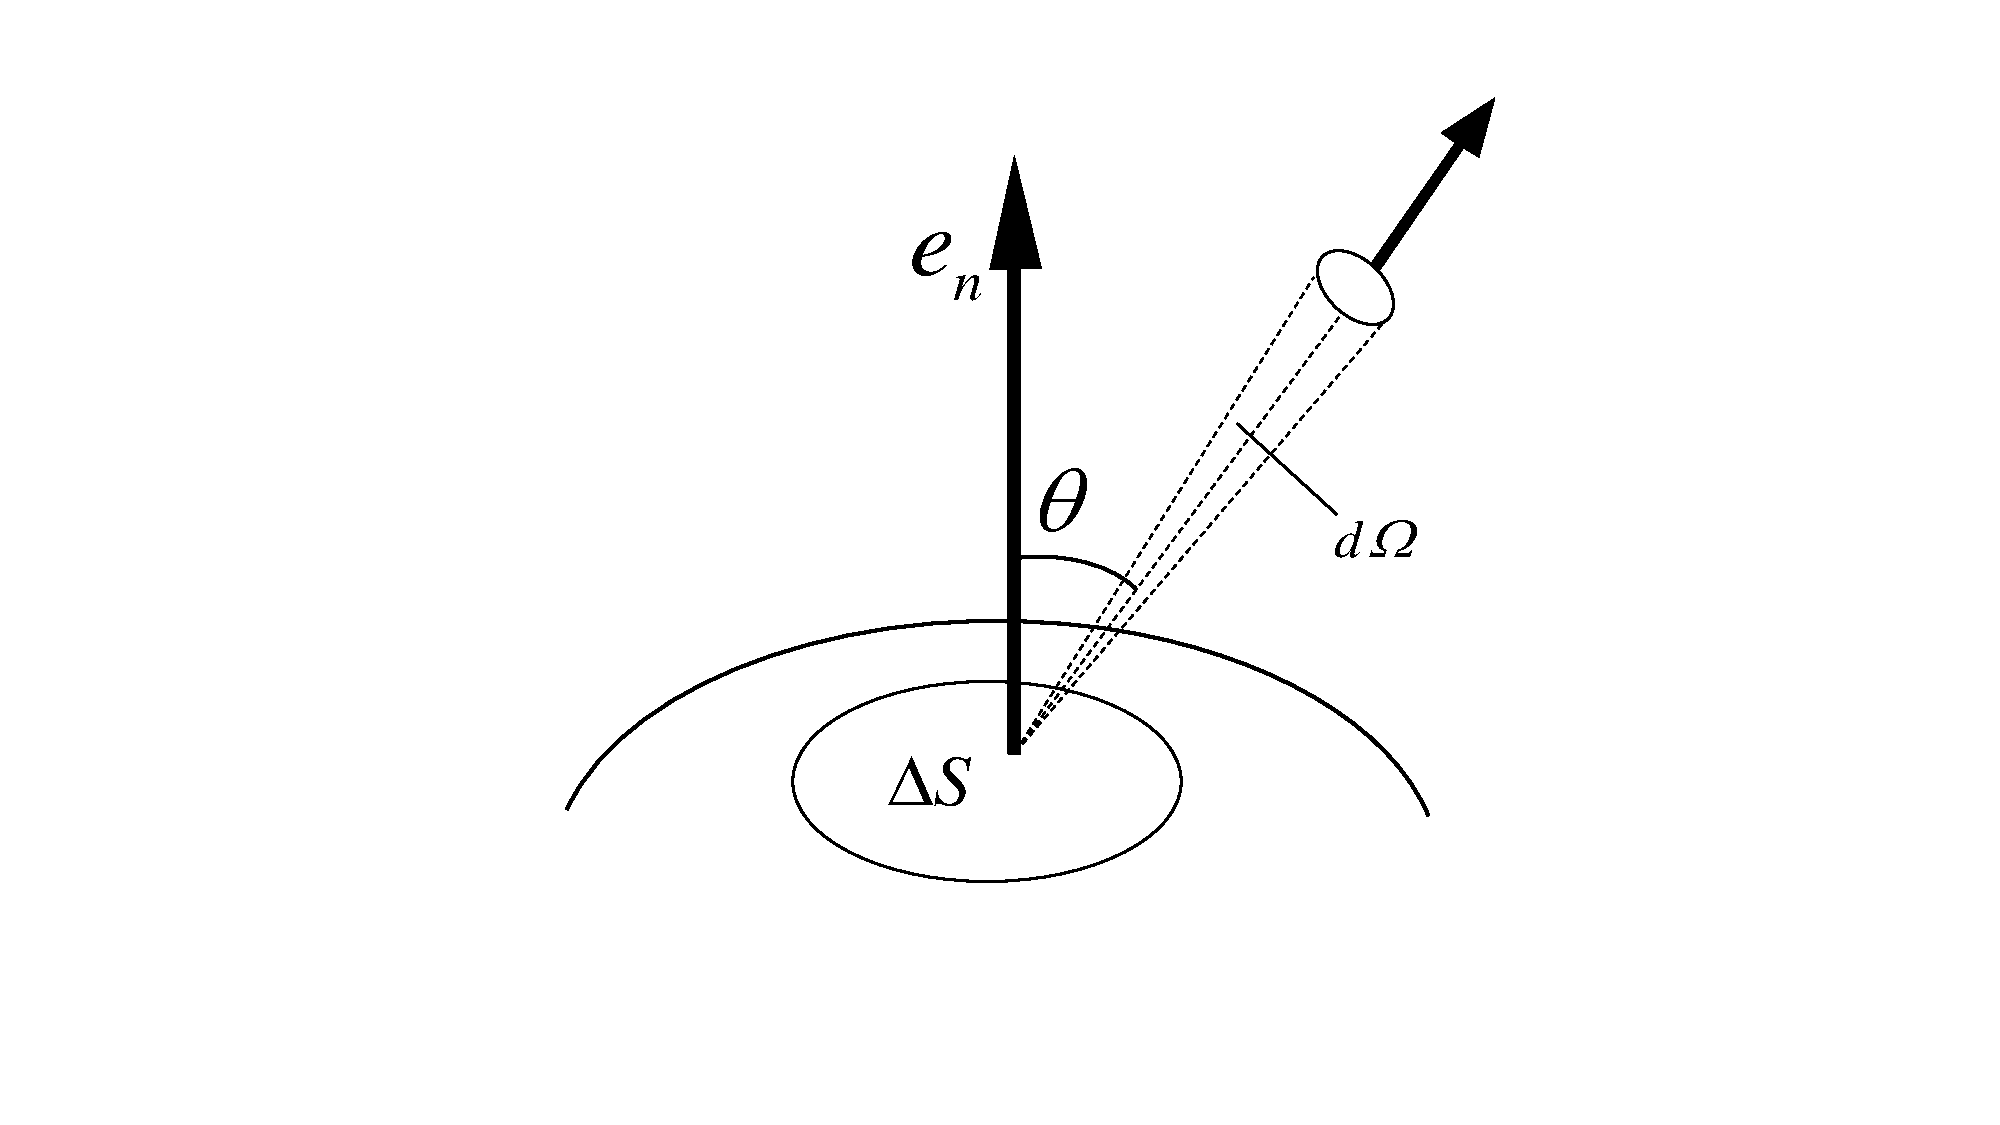
\includegraphics[width=2.5cm]{QM file/figure/1-1}
	\caption{}\label{fig.1-1}
\end{wrapfigure}
\eqindent{4}
\begin{equation*}
	\sigma=5.6704 \times 10^{-8} \si{W\cdot m^{-2} \cdot K^{-4}} 
\end{equation*}\eqnormal

图\ref{fig.1-1}是黑体辐射示意图,将空腔加热至温度$T$,这时腔内电磁场具有稳定的能量分布(各种频率的电磁波),经由小孔 $\Delta S$辐射出的能流可用仪器测出.如以$u$表示腔内电磁场能量密度(单位体积内电磁波能量),$c$表示光速,则单位时间内由$\Delta S$沿$d \Omega$方向辐射出的能量为
\begin{equation*}
	\Delta S\cdot \cos\theta\cdot cu\frac{d\Omega}{4\pi}
\end{equation*}
经$\Delta S$辐射出的总能量为
\begin{equation*}
	\begin{aligned}
		J_{u}\Delta S &=\int_{\theta \leq\frac{\pi}{2}}\Delta S \cos\theta cu \frac{d\Omega}{4\pi} \\
		&=\Delta S cu\frac{1}{4\pi}\int_{0}^{2\pi}d\varphi \int_{0}^{\frac{\pi}{2}}\cos\theta\sin\theta d\theta \\
		&= \frac{1}{4}cu\Delta S \\
	\end{aligned}
\end{equation*}
因此
\eqshort
\begin{equation}\label{eq11.02}
	u=\frac{4}{c}J_{u}=\frac{4\sigma}{c}T^{4}
\end{equation}
热辐射电磁场的能量密度与温度4次方成正比.注意比例系数为普适常数.

实验还可以测量出热辐射能量的频率分布.电磁波的波长$\lambda$与频率$\nu$及角频率$\omega=2\pi\nu$间有如下关系:
\begin{equation}\label{eq11.03}
	c=\lambda\nu=\frac{\lambda \omega}{2\pi}
\end{equation}
如以$\rho(\omega)d\omega$表示单位体积内角频率在$(\omega,\omega+d\omega)$间的电磁波能量,则能量密度$u$按$\omega$分布可以表示成
\begin{equation}\label{eq11.04}
	u=\int_{0}^{u} \rho(\omega)d\omega
\end{equation}\eqnormal
\begin{wrapfigure}[9]{r}{9em}
	\centering
	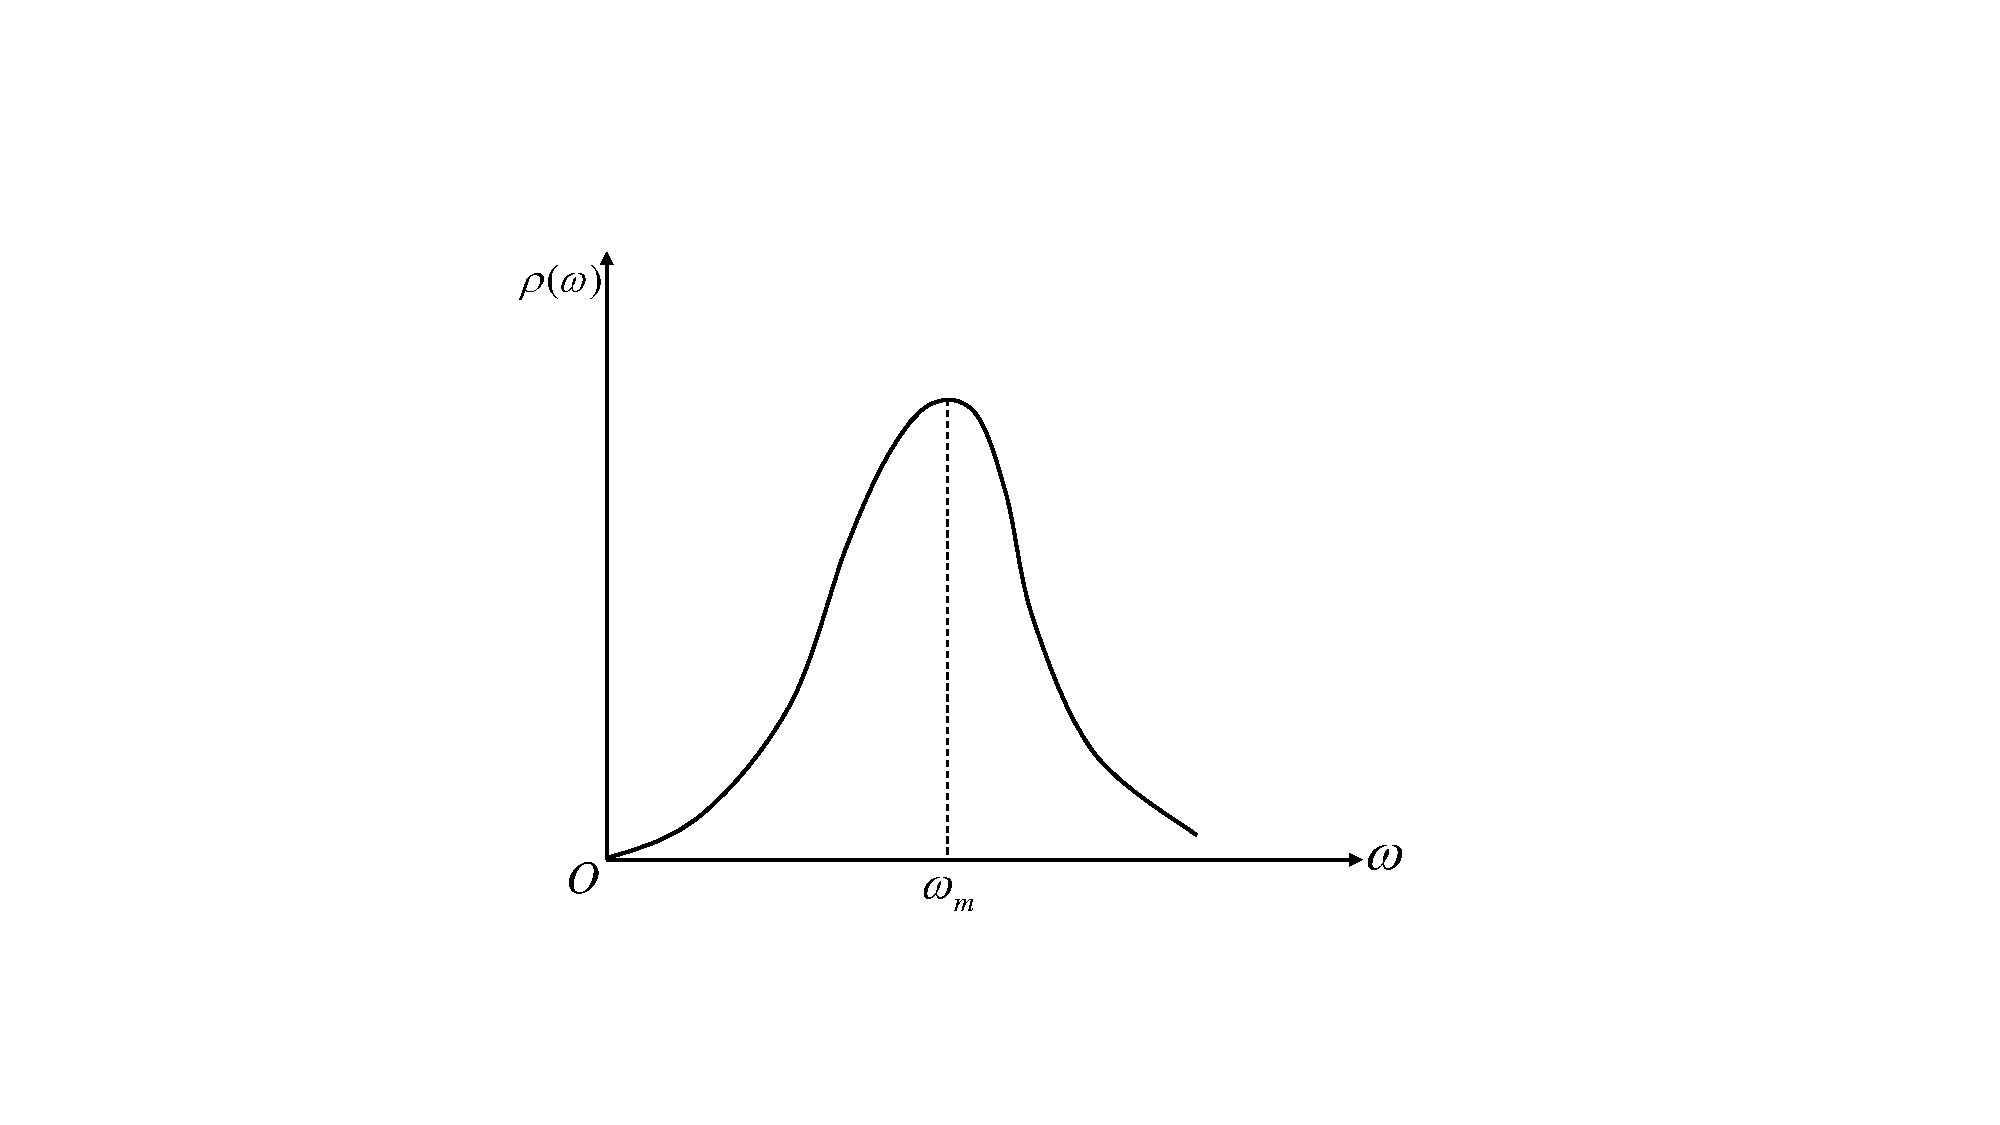
\includegraphics[width=3.5cm]{QM file/figure/1-2}
	\caption{}\label{fig.1-2}
\end{wrapfigure}

实验测得各种温度下$u$的频率分布曲线如图\ref{fig.1-2}所示.在长波部分$(\omega \rightarrow 0)\rho(\omega)\propto \omega^{2}T$;在短波部分$(\omega\rightarrow\infty)\rho(\omega)$随$\omega$之增大而迅速减小.对于每一种温度,$\rho(\omega)$都存在一个极大值,相应的角频率$\omega_{m}$和温度$T$成正比,相应的波长$(\lambda_{m}=\frac{2\pi c}{\omega_{m}})$和温度$T$成反比,
\eqindent{5}
\begin{equation}\label{eq11.05}
	T\lambda_{m}=5.1\times 10^{-3}  \si{m\cdot K}
\end{equation}\eqnormal
这规律称为维恩(W.Wein)位移定律.注意\eqref{eq11.05}式中的实验常数也是普适常量.

黑体辐射定律的发现引起了物理学界的极大关注,吸引力许多著名学者对它进行深入的理论探讨.当时经典物理学(牛顿力学,电磁学,热力学和经典统计物理是其主要内容)已经日臻成熟,权威物理学家大多相信经典物理学能够解释各类物理现象,黑体辐射定律应该也不例外.然而,冷酷的事实确是,企图在经典物理的理论框架内解释黑体辐射定律的努力,都在不同程度上遭到失败,其中最有成效的是瑞利和金斯(Rayleigh-Jeans)的研究.金斯利用波动理论,准确求得单位体积内$(\omega,\omega+d\omega)$范围内电磁振动模式总数,它等于
\eqindent{12}
\begin{equation}\label{eq11.06}
	\frac{\omega^{2}d\omega}{\pi^{2}c^{3}}
\end{equation}
\eqnormal
每一种电磁振动模式相当于一个简谐振子,在温度$T$下应该具有某种能量.按照经典统计物理的“能量均分定理”,温度$T$下简谐振子应该具有平均能量$kT$(k是玻尔兹曼常数).瑞利将“能量均分定理”用于热平衡下的电磁场(即热辐射场),从而得出结论:单位体积内$\omega,\omega+d\omega$范围内电磁振动能量应该是
\begin{equation}\label{eq11.07}
	\rho(\omega)d\omega=\frac{kT\omega^{2}d\omega}{\pi^{2}c^{3}}
\end{equation} 
这称为瑞利-金斯公式.这个公式在长波部分和实验曲线符合得极好,而在短波部分则和实验结果完全不符合.更严重的是,\eqref{eq11.07}式对$\omega$积分,将导致$u\rightarrow\infty$,这个结论显然是错误的.这就是历史上有名的“紫外发散困难”.

经历了许多失败,终于使物理学界认识到,为了解释黑体辐射定律,光靠经典物理学是不行的,必须有一个新的理论.这就是1900年普朗克(M.Planck)提出的量子论.

普朗克量子论的核心是下述“量子假设”:频率为$\nu$的电磁振动和原子、分子等物质发生能量转换时,能量不能连续变化,只能“量子”式地变化,每份“能量子”为
\begin{equation}\label{eq11.08}
	\varepsilon=h\nu=\hbar\omega \quad(\hbar=\frac{h}{2\pi})
\end{equation}
其中$h$是普适常数(后人称之为普朗克常数).在这假设下,普朗克利用热力学和统计物理理论,导出了著名地普朗克公式
\begin{equation}\label{eq11.09}
	\boxed{\rho(\omega)=\frac{\hbar\omega^{3}}{\pi^{2}c^{3}} \bigg/ (e^{\hbar\omega/kT}-1)}
\end{equation}

这个公式在各种温度下,全部频率范围内,均与实验曲线精确符合.历史上,普朗克导出\eqref{eq11.09}式的过程相当复杂.$\S$\ref{sec:09.04}将给出爱因斯坦对此式的简单证明.

普朗克的“量子假设”是和经典物理的整套概念抵触的.按照经典物理学,一切物质的运动变化都是连续进行的,能量变化也是连续的,这正是导致热平衡下“能量均分定理”的前提条件.普朗克舍弃了“能量均分定理”,代之以“量子假设”这在概念上是一次革命性的突破.从\eqref{eq11.09}式的结果看,由于能量的量子化,角频率为$\omega$的每一种电磁振动模式在温度$T$下的平均能量不再取“能量均分定理”给出的$kT$,而是
\begin{equation*}
	 E_{\omega}=\frac{\hbar\omega}{e^{\hbar\omega/kT}-1} 
\end{equation*}
在长波部分,$\hbar\omega\ll kT$,上式给出$\bar{E}_{\omega}\simeq kT$,与能量均分定理的结论一致.在短波部分,$\hbar\omega\gg kT$,上式给出
\begin{equation*}
	 \bar{E}_{\omega}\simeq \hbar\omega e^{\hbar\omega/kT} \ll kT 
\end{equation*}
这意味着高频振动被“冻结”,很难获得能量,因此避免了“紫外发散困难”.当一种电磁振动模式(角频率$\omega$)具有能量$E_{\omega}$时,相应的“能量子”数目为$n_{\omega}=\frac{E_{\omega}}{\hbar\omega}$,\eqref{eq11.09}式相当于“能量子”数的平均值为
\eqshort
\begin{equation}\label{eq11.10}
	\bar{n}_{\omega}=\frac{1}{e^{\hbar\omega/kT}-1}
\end{equation}
当$\hbar\omega\ll kT$,$\bar{n}_{\omega}=\simeq\frac{kT}{\hbar\omega}\gg 1$,电磁振动的能量变化近似于连续变化,量子论的结果和经典物理结果一致,当$\hbar\omega\gtrsim kT$,$\bar{n}_{\omega}<1$,量子论的结果和经典物理结果有本质差别.

\eqref{eq11.09}式代入\eqref{eq11.04}式,可以算出热辐射电磁场能量密度:
\begin{equation}\label{eq11.11}
	u=\frac{\pi^{2}(kT)^{4}}{15(\hbar c)^{3}}
\end{equation}\eqnormal
这结果与斯特藩-玻尔兹曼定律一致.

普朗克的“量子假设”是与整个经典物理格格不入的,使许多习惯于经典物理思维模式的资深物理学家感到难以接受.普朗克本人就曾花了多年时间研究能否不要“量子假设”,而在经典物理的范围内导出\eqref{eq11.09}式,结论是不能.显然,这意味着黑体辐射现象的后面隐藏着一种新的物理规律,这就是今天所谓的量子力学规律.

在这里,我们将用量纲分析方法证明黑体辐射定律绝不可能在经典物理学的框架范围内得到解释.

物理学的发展历史表明,每一种基本物理规律,均伴有相应的普适常数.例如代表万有引力定律的普适常数是引力常数$G$,代表电磁规律和相对论的基本普适常数是光速$c$,代表统计物理规律的基本普适常数是玻尔兹曼常数$k$,等等.如果黑体辐射定律可由经典物理来解释,有关的理论将是电磁学和统计物理,则在辐射场能量密度$u$的构造式中,只能包含$c,k,T$ $L,t,E,K$分别表示长度,时间,能量,温度的量纲,有关各量的量纲如下:
\begin{gather*}
	u——  \si{EL^{-3}},\qquad \qquad c——  \si{Lt^{-1}}  \\
	k——  \si{EK^{-1}},\qquad \qquad kT—— \si{E}  \\
	\sigma——  \si{Et^{-1}L^{-2}K^{-4}}
\end{gather*}
从量纲关系看,$u$显然不能由$c,k,T$构成,$\sigma$(普适常数)不可能由$c,k$构成.根据\eqref{eq11.02}式,可以判断$u\propto(kT)^{4}$,而从$u,c$与长度的量纲关系来看,可以设想$u\propto c^{-3}$,因此,$u\propto(kT)^{4}c^{-3}$.而$uc^{3}(kT)^{-4}$的量纲为$\si{(Et)^{-3}}$.如果设想黑体辐射现象涉及一种新的(未知的)基本物理规律,相应的基本普适常量(记为$\hbar$)量纲为$\si{Et}$,则$u$的构造式可以设想为
\eqshort
\begin{equation}\label{eq11.12}
	u=A(kT)^{4}(\hbar c)^{-3}
\end{equation}
其中$A$为无量纲纯数,结合\eqref{eq11.02}式,可得斯特藩-玻尔兹曼常数的构造式为
\begin{equation}\label{eq11.13}
	\sigma=\frac{A}{4}k^{4}\hbar^{-3}c^{-2}
\end{equation}\eqnormal
读者当然已经想到,这里提到的代表新规律的基本普适常数$\hbar$正好就是普朗克常数.事实上,如略去\eqref{eq11.12}、\eqref{eq11.13}式中不太重要的纯数$A$,利用$c,k,\sigma$的实验值,由\eqref{eq11.13}式即可估算出$\hbar \sim1.2\times 10^{-34} \si{J\cdot s}$,这正是普朗克常数$\frac{h}{2\pi}$的量级.如按精确计算得到的\eqref{eq11.11}式,[相当于\eqref{eq11.12}、\eqref{eq11.13}式中取$A=\frac{\pi^{2}}{15}$]则如上所述可以算出
\setlength{\mathindent}{4em}
\begin{equation*}
	\hbar=1.0546\times 10^{-34} \si{J\cdot s},\quad h=2\pi\hbar=6.6262\times 10^{-34} \si{J\cdot s}
\end{equation*}
\setlength{\mathindent}{9em}
这数值与普朗克常数的精密测量值非常接近.

\example 试用普朗克公式\eqref{eq11.09}求$\rho(\omega)$极大值对应的角频率$\omega_{m}$与温度$T$的数值关系,并估算热辐射场的光子数密度.

\solution $\rho(\omega)$取极大值时,满足极值条件$\frac{\partial \rho}{\partial \omega}=0$.令$x=\frac{\hbar\omega}{kT}$,极值条件亦即
\eqshort
\begin{equation*}
	\frac{d}{dx}\frac{x^{3}}{e^{x}-1}=0
\end{equation*}
由此得出$x$满足的方程为
\begin{equation*}
	\frac{x}{3}=1-e^{-x}
\end{equation*}
用数值解法可解出$x=\num{2.8214}$,因此
\begin{equation}\label{eq11.14}
	\frac{\hbar\omega_{m}}{kT}=\num{2.8214}
\end{equation}\eqnormal
这正是维恩位移定律.读者不难验证\eqref{eq11.14}式与\eqref{eq11.05}式是一致的.

由于辐射场的能量集中分布在$\omega\sim\omega_{m}$附近,所以光子数密度(单位体积内光子数)可估计成
\begin{equation}\label{eq11.15}
	n\sim\frac{u}{\hbar\omega_{m}}\sim\frac{\pi^{2}}{15\times2.82}\bigl(\frac{kT}{\hbar c}\bigr)^{3}\sim 0.23\bigl(\frac{kT}{\hbar c}\bigr)^{3}
\end{equation}
精确结果是
\begin{equation}\label{eq11.16}
	n=\int_{0}^{\infty}\frac{\rho(\omega)}{\hbar\omega}d\omega=0.2436\bigl(\frac{kT}{\hbar c}\bigr)^{3}
\end{equation}

从量纲关系看,$n$的构造式中只能包含$kT,c,\hbar$,他们的量纲是
\begin{equation*}
	n——\si{L^{-3}},\quad kT—— \si{E},\quad \hbar c—— \si{EL} 
\end{equation*}
所以唯一可能的量纲构造关系是$n\sim\bigl( \frac{kT}{\hbar c} \bigr)^{3}$









% 光子
\section[光子]{\makebox[5em][s]{光子}}\label{sec:01.02}
% \makebox[5em][s]{} % 短题目拉间距
% \setlength{\mathindent}{9em} 本文标准公式缩进

1905年,爱因斯坦将普朗克的量子假设发展成光量子(光子)的概念也正是这一年,爱因斯坦创立了狭义相对论.

爱因斯坦认为,电磁波(光波)的结构应该是量子化的,其最小单元即一个光子,每个光子均以同样的速度$c$(光速)运动频率为$v$的光波,其光子的能量和动量为
\begin{align}
	E=h\nu=\hbar\omega \label{eqn:01.02.01} \\ 
	p\approx \frac{E}{c}=\frac{h\nu}{c}=\frac{h}{\lambda} \label{eqn:01.02.02}
\end{align}
$\lambda$为光波的波长,光子的运动方向应该和光波的传播方向一致.

对于单色平面波,如引入“波矢量”$\boldsymbol{k}$,其方向为波的传播方向,其数值为$k=| \boldsymbol{k}|=\frac{2\pi}{\lambda}$,则光子的动量可以表示成
\eqindent{12}
\begin{equation}\label{eqn:01.02.03}
	\boldsymbol{p}=\hbar \boldsymbol{k}
\end{equation}\eqnormal

光和其他物质发生相互作用时,基元过程通常表现为光子-电子作用或者光子-原子作用,利用光子的概念并对作用过程应用能量守恒定律,一般就能够得出某些(但不是全部)重要结论.

\textsf{1. 光电效应}

某些金属受到光的照射后,能够发射出电子,形成电流,这就是光电效应其物理机理可用光子概念解释如下金属中的“自由电子”要逸出金属表面,需要克服“逸出功”,$W$当金属受到频率为$v$的光照射时,自由电子即可吸收光子,从而获得能量(电子同时或在短时间内连续吸收两个以上光子的机会极小,可以不考虑这种可能性.)如$h\nu>W$,电子就可以从金属中逸出,并具有动能
\begin{equation}\label{eqn:01.02.04}
	\boxed{\frac{1}{2}m_{c}v^{2}=h\nu-W}
\end{equation}
由此可见,光电子的动能完全由逸出功$W$(由金属性质决定)和入射光的频率$v$所决定,而与光的强度无关光电子的数目则与入射光的强度成正比,即和入射光子的总数成正比对光电子动能的实验测量完全证实了爱因斯坦公式\eqref{eqn:01.02.04}的正确性由\eqref{eqn:01.02.04}式还可看出,当逸出功$W$给定后,入射光的频率$v$必须超过$W/h$,才能产生光电效应;如$v<\frac{W}{h}$,尽管光很强,也不会产生光电子这个结论也已为实验证实.

\textsf{2. 康普顿散射}

关于光子能量和动量的爱因斯坦公式\eqref{eqn:01.02.01}、\eqref{eqn:01.02.03},于l923年被康普顿(A.H.Compton)散射所证实实验发现,X射线被石蜡等轻物质散射时,波长增大经典电磁理论很难解释这现象康普顿利用光子的概念,并假定在光子-电子作用过程中,能量守恒定律和动量守恒定律成立,利用相对论力学,对散射过程作出了成功的理论分析.

$X$射线的光子能量,约在$10^{3}\si{eV}$以上轻物质中外层电子的原子能级仅几个电子伏,可以当作自由电子设$X$射线的入射波长为$\lambda$,则入射光子的能量、动量为
\begin{equation} 
	\begin{aligned} \notag
		E=h\nu=\frac{hc}{\lambda} \\
		p=\frac{E}{c}=\frac{h\nu}{c}=\frac{h}{\lambda}
	\end{aligned}
\end{equation}
\begin{wrapfigure}[7]{r}{9em}
	\centering
	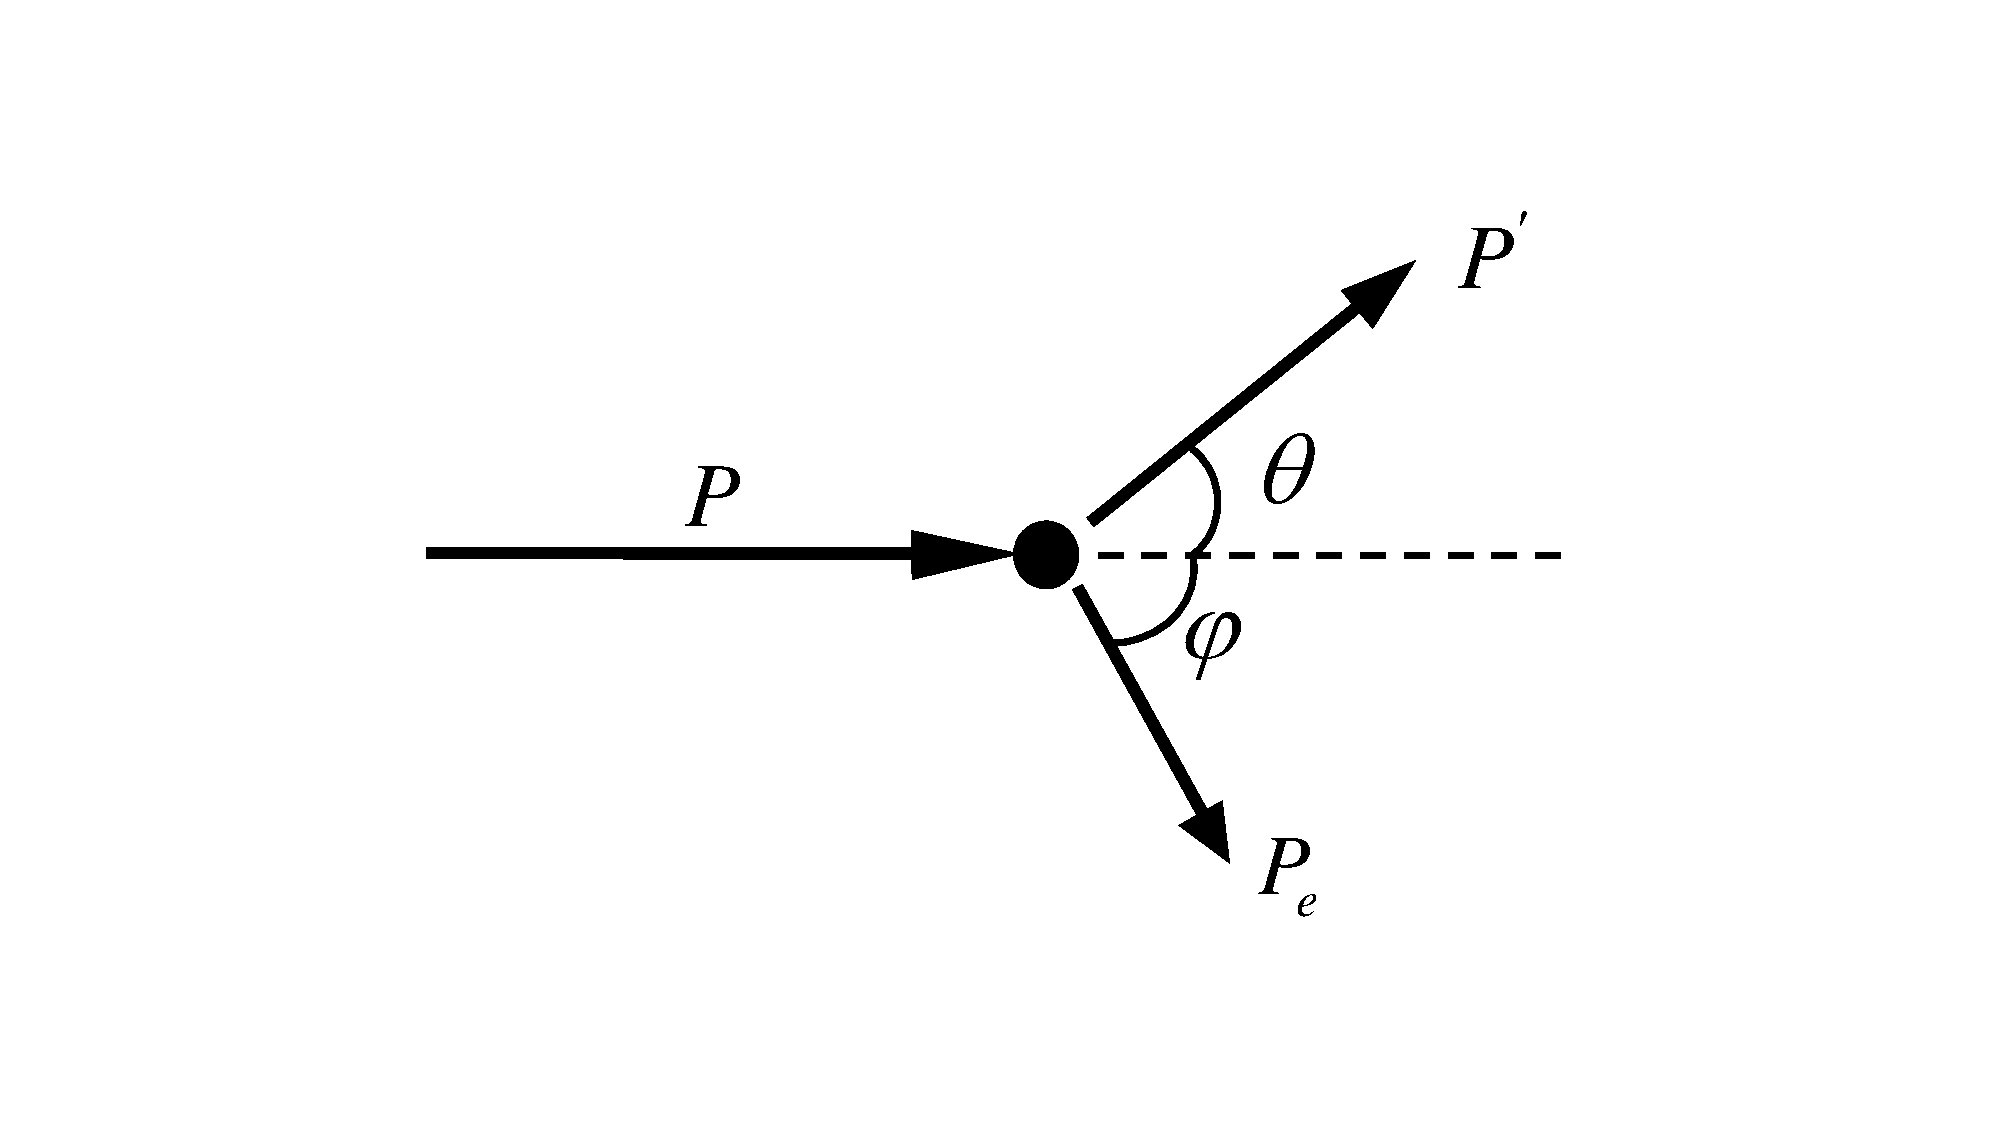
\includegraphics[width=3cm]{QM file/figure/1-3}
	\caption{}
	\label{fig.1-3}
\end{wrapfigure}
电子初始动量为0,初始能量为$m_{c}c^{2}$散射(碰撞)后,设光子沿$\theta$方向射出,如图\ref{fig.1-3},波长变为$\lambda^{\prime}$,能量及动量变为
\setlength{\mathindent}{6em}
\begin{equation}
	\begin{aligned} \notag
		E^{\prime}=h\nu^{\prime}=\frac{hc}{\lambda^{\prime}} \\
		p^{\prime}=\frac{E^{\prime}}{c}=\frac{h\nu^{\prime}}{c}=\frac{h}{\lambda^{\prime}}
	\end{aligned}
\end{equation}
\eqnormal
电子的反冲角设为$\varphi$能量和动量设为$E_{e}$和$p_{e}$,按照相对论力学
\begin{equation}\label{eqn:01.02.05}
	E_{e}^2=c^{2}p_{e}^{2}+m_{e}^{2}c^{4}
\end{equation}
对散射过程应用能量守恒定律,得到
\begin{equation*}
	h\nu+m_{e}c^{2}=h\nu^{\prime}+E_{e}^{2}
\end{equation*}
亦即
\begin{equation}\label{eqn:01.02.06}
	h(\nu-\nu^{\prime})=E_{e}-m_{e}c^{2}
\end{equation}
对散射过程应用动量守恒定律,得到
\begin{equation}\label{eqn:01.02.07}
	\boldmath p-p^{\prime}=p_{e}
\end{equation}
取平方,得到
\begin{equation*}
	p^{2}+p^{\prime 2}-2\boldsymbol{p}\cdot\boldsymbol{p^{\prime}}=p_{e}^{2}
\end{equation*}
亦即
\begin{equation}\label{eqn:01.02.08}
	h^{2}(\nu+\nu^{\prime}-2\nu\nu^{\prime}\cos\theta)=E_{e}^{2}-m_{e}^{2}c^{4}
\end{equation}
\eqref{eqn:01.02.06}式取平方,则得
\begin{equation*}
	h^{2}(\nu+\nu^{\prime}-2v\nu^{\prime})=(E_{e}-m_{e}c^{2})^{2}
\end{equation*}
与\eqref{eqn:01.02.08}式相消,得到
\begin{equation}
	\begin{aligned}
		2h^{2}\nu\nu^{\prime}(1-\cos\theta) &=2m_{e}c^{2}(E_{e}-m_{e}c^{2}) \\
		&=2m_{e}c^{2}h(\nu-\nu^{\prime})
	\end{aligned}
\end{equation}
因此,
\begin{equation*}
	\frac{1}{\nu}-\frac{1}{\nu^{\prime}}=\frac{h}{m_{e}c^{2}}(1-\cos\theta)
\end{equation*}
亦即
\begin{equation}\label{eqn:01.02.09}
	\boxed{\lambda^{\prime}-\lambda=\frac{h}{m_{e}c}(1-\cos\theta)}
\end{equation}
经过散射,X射线得波长有所增加,增量$(\lambda^{\prime}-\lambda)$与散射角有关,并与$\frac{h}{m_{e}c}$成比例,后者称为康普顿波长,记为$\lambda_{c}$,
\begin{equation}\label{eqn:01.02.10}
	\lambda_{c}=\frac{h}{m_{e}c}=2.43\times10^{-12} \si{m}
\end{equation}
对散射光波长的实验证实了\eqref{eqn:01.02.09}式的正确性因此,康普顿散射证实了:(i)光子的能量、动量公式\eqref{eqn:01.02.01}、\eqref{eqn:01.02.02}、\eqref{eqn:01.02.03}是正确的;(ii)微观基元过程中,能量守恒定律和动量守恒定律成立;(iii)相对论力学是正确的.

\textsf{3. 粒子-反粒子对的湮没与产生}

实验发现,电子($e^{-}$)及其反粒子(正电子,$e^{+}$)相碰,可以湮没而产生两个$\gamma$光子,即
\begin{equation*}
	e^{-}+e^{+}\rightarrow \gamma+\gamma
\end{equation*}
根据相对论力学及能量、动量守恒定律,每个$\gamma$光子的能量至少等于电子的静能,即$E_{r}\geqslant m_{e}c^{2}$,相应的$\gamma$射线波长为
\begin{equation*}
	\lambda=\frac{hc}{E_{r}}\leqslant\frac{h}{m_{e}c}=\lambda_{c}
\end{equation*}
这个关系已为实验所证实粒子物理的理论分析表明,能够产生上述湮没过程的电子、正电子距离,大致也是康普顿波长的量级.

在温度$T$下,热辐射光子的平均能量约为$3kT$(k为玻尔兹曼常数)按照近代天体物理理论,在宇宙形成的初期,温度极高,两个光子相碰,可能转变成(质子、反质子)对或(中子,反中子)对,按照能量守恒定律,有
\begin{equation*}
	E_{\gamma}\approx3kT\approx m_{p}c^{2}=938 \si{MeV}
\end{equation*}
因此当时温度约为
\begin{equation*}
	T\approx m_{p}c^{2} \big/ 3k\approx3.6\times10^{12} \si{K}
\end{equation*}




% 玻尔的量子论
\section[玻尔的量子论]{玻尔的量子论}\label{sec:01.03}
% \makebox[5em][s]{} % 短题目拉间距
% \setlength{\mathindent}{9em} 本文标准公式缩进 
% \eqnormal % 恢复标准缩进

\textsf{1. 氢原子光谱}

19世纪后期,广泛进行了原子光谱的实验研究.1885年,巴尔末(Balmer)在氢原子光谱中发现了一个谱线系,其频率可以精确地表示成
\begin{equation}\label{eqn:01.03.01}
	\nu=\frac{c}{\lambda}=cR\bigg( \frac{1}{2^2}-\frac{1}{n^2} \bigg),\quad n=3,4,5,\cdots
\end{equation}
其中
\begin{equation*}
	R=\num{10967758.1} \si{m^{-1}} \text{(里德伯常数)}
\end{equation*}
后来又发现了其他谱线系.总的说,氢原子光谱全部谱线的频率可以归结成公式
\setlength{\mathindent}{6em}
\begin{equation}\label{eqn:01.03.02}
	\nu=\frac{c}{\lambda}=cR\bigg( \frac{1}{m^2}-\frac{1}{n^2} \bigg),\quad m<n \text{($m,n$为正整数)}
\end{equation}
\eqnormal
光谱公式虽然是经验公式,但是其精确度极高,为任何其他定量公式所不及.因此有理由相信,在这些公式后面一定隐藏着某种深刻的物理规律.

\textsf{2. 卢瑟福原子模型}

\begin{wrapfigure}[7]{r}{6em}
	\centering
	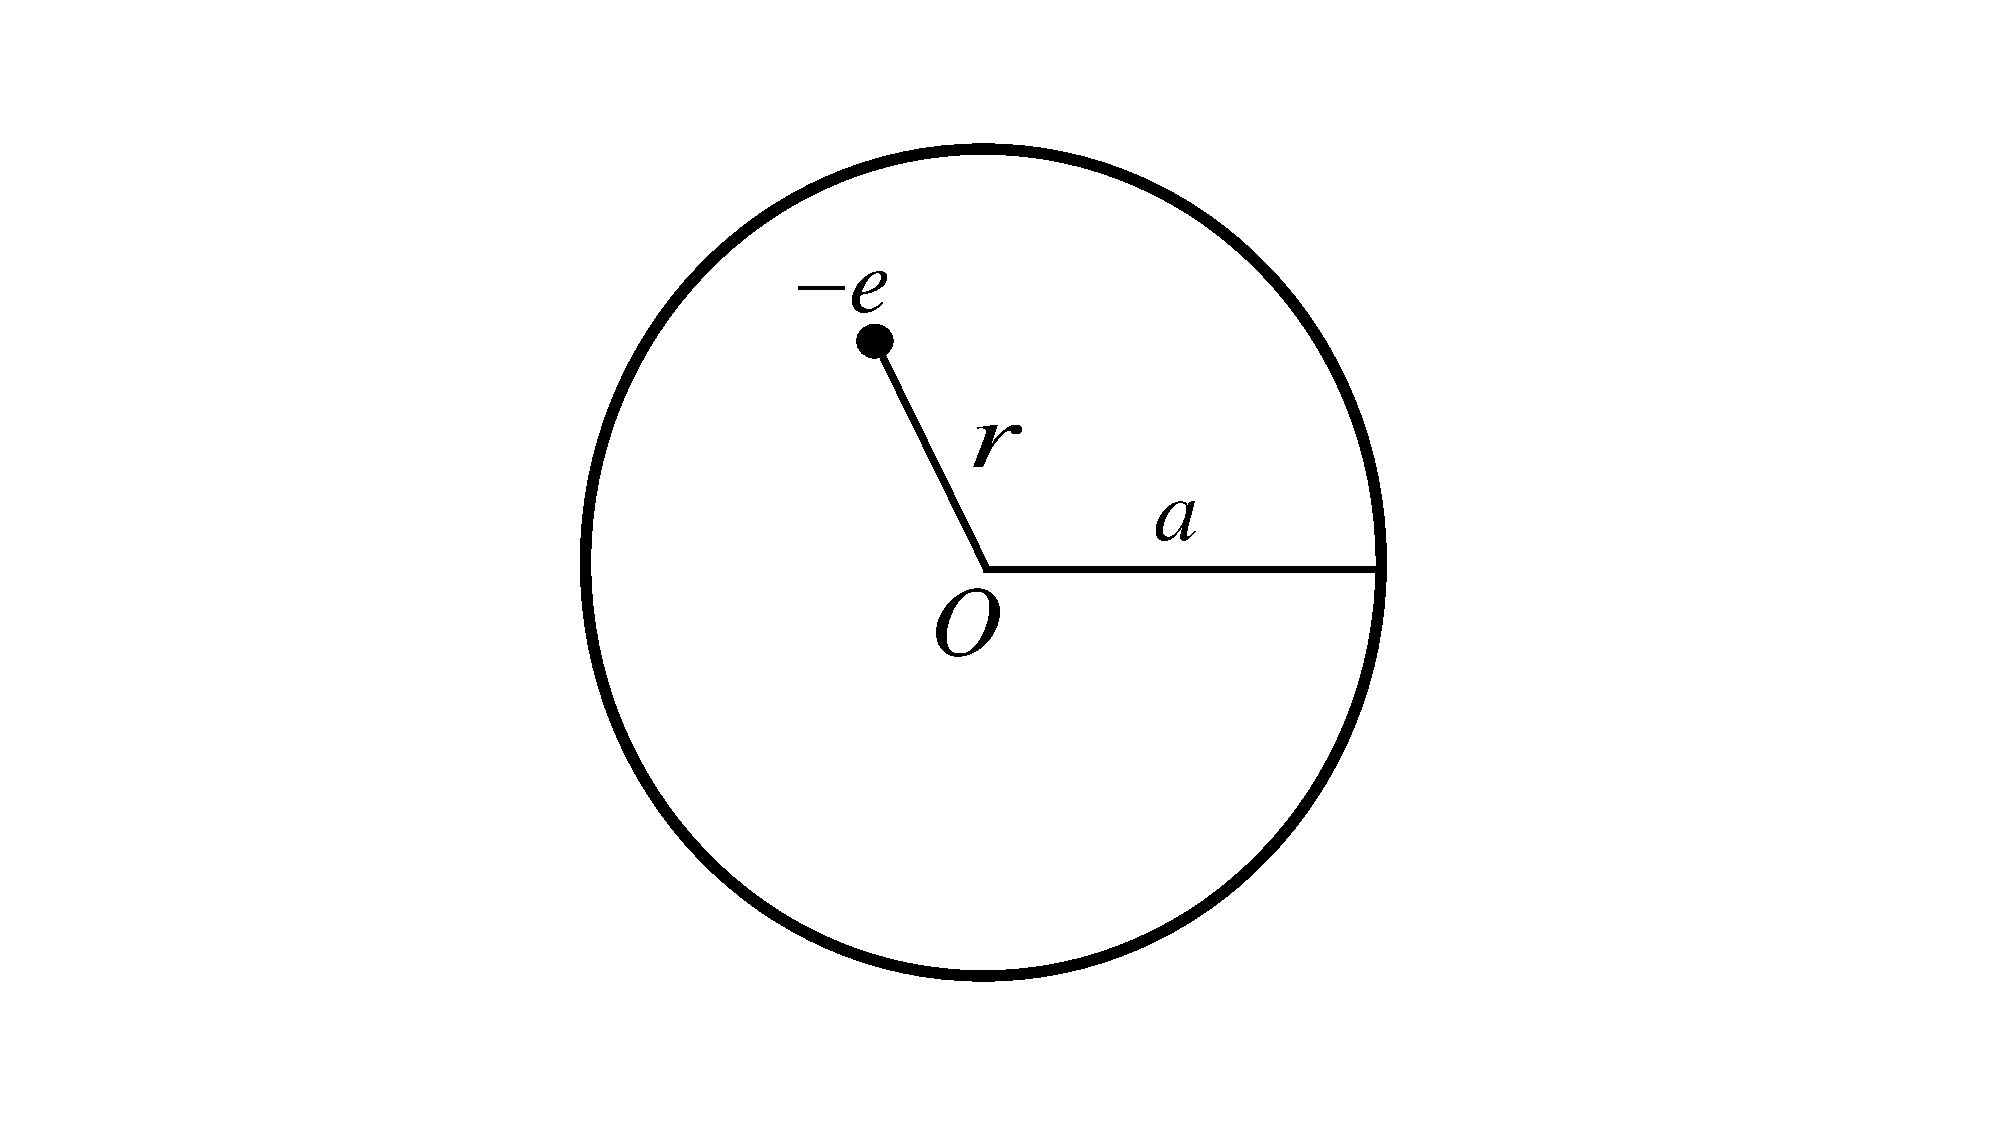
\includegraphics[width=2cm,clip]{QM file/figure/1-4}
	\caption{}
	\label{fig.1-4}
\end{wrapfigure}
1897年,汤姆孙(J.J.Tomson)用测量荷质比$\frac{e}{m_{e}}$的办法发现了电子.1903年,他顺理成章地提出了一种原子模型:原子的质量及正电荷均匀分布在球形体积中,球的半径即原子半径.电子(质量为$m_{e}$,远小于原子质量)在正电荷的库仑力作用下,可在原子内运动.按照汤姆孙原子模型,正常情况下电子停留在原子中心(球心),这时原子不发光.如因外力作用而使电子偏离了原子中心,正电荷对电子的库仑作用力将使电子在中心附近作简谐振动,从而向外辐射电磁波,即原子将发光.以单电子原子为例,如\ref{fig.1-4}所示,正电荷$Q=e$均匀分布在球内,电子(电荷$q=-e$)偏离球心时,库仑力为
\eqlong
\begin{equation}\label{eqn:01.03.03}
	\boldsymbol{F}=\-\frac{e^{2}}{4\pi\varepsilon_{0}}\bigg(\frac{r}{a} \bigg)^{3} \frac{r}{r^{3}}=-\frac{e^{2}}{4\pi\varepsilon_{0}}\frac{r}{a^{3}}
\end{equation}\eqnormal
今后,凡涉及库仑力问题,公式中$4\pi\varepsilon_{0}$一律省略不写.$\frac{e^{2}}{4\pi\varepsilon_{0}}$简记为$\e^{2}$.\eqref{eqn:01.03.03}式简写成
\eqshort
\begin{equation*}\label{eqn:01.03.03'}
	\boldsymbol{F}=-\frac{\e^{2}}{a^{3}} \boldsymbol{r} \tag{$1.3.3^{\prime}$}
\end{equation*}\eqnormal
库仑力表现为弹性力,因此电子将在球心附近作简谐运动,频率为
\eqlong
\begin{equation}\label{eqn:01.03.04}
	\nu=\frac{\omega}{2\pi}=\frac{1}{2\pi}\bigg(\frac{\e^2}{m_{e}a^3} \bigg)^{\frac{1}{2}}=\frac{1}{2\pi a}\bigg(\frac{\e^2}{m_{e}a^3} \bigg)^{\frac{1}{2}}
\end{equation}
电子振动时,将辐射出同样频率的电磁波,波长为
\begin{equation}\label{eqn:01.03.05}
	\lambda=\frac{c}{\nu}=2\pi ac\bigg(\frac{m_{e}a}{\e^2} \bigg)^{\frac{1}{2}}=2\pi a\bigg(\frac{a}{r_{e}} \bigg)^{\frac{1}{2}}
\end{equation}
其中为c光速,$r_{e}$为“经典电子半径”,
\begin{equation}\label{eqn:01.03.06}
	r_{e}=\frac{\e^2}{m_{e}c^{2}}=2.82\times10^{-15} \si{m}=2.82 \si{fm}
\end{equation}\eqnormal
如取原子半径$a\sim 0.1 \si{nm}=10^{-10} \si{m}$,求出
\begin{equation*}
	\lambda \sim 118 \si{nm},\quad \nu\sim 2.5\times10^{15} \si{s^{-1}}
\end{equation*}
属于紫外光区域.从数量级说,和原子光谱的范围大体相符.但是这种原子模型显然无法解释实验已经发现的氢原子光谱公式\eqref{eqn:01.03.02}.

汤姆孙原子模型终于被否定,是由于卢瑟福(Rutherford)的$\alpha$粒子对重元素的散射实验(1912)结果.

来自元素天然放射性的$\alpha$粒子,质量约为电子的7000倍,但比重元素的原子轻得多.因此在散射过程中,原子可以近似地当作是静止的.$\alpha$粒子的实验室动能约为几个$\si{MeV(10^{6} \si{eV})}$,远大于原子中电子的电离能(数量级$10\si{eV}$),因此当$\alpha$粒子与电子的距离接近到原子半径的量级时,即可使电子电离.只有原子中的正电荷才是使$\alpha$粒子发生散射的主要因素.

\begin{wrapfigure}[6]{r}{6em}
	\centering
	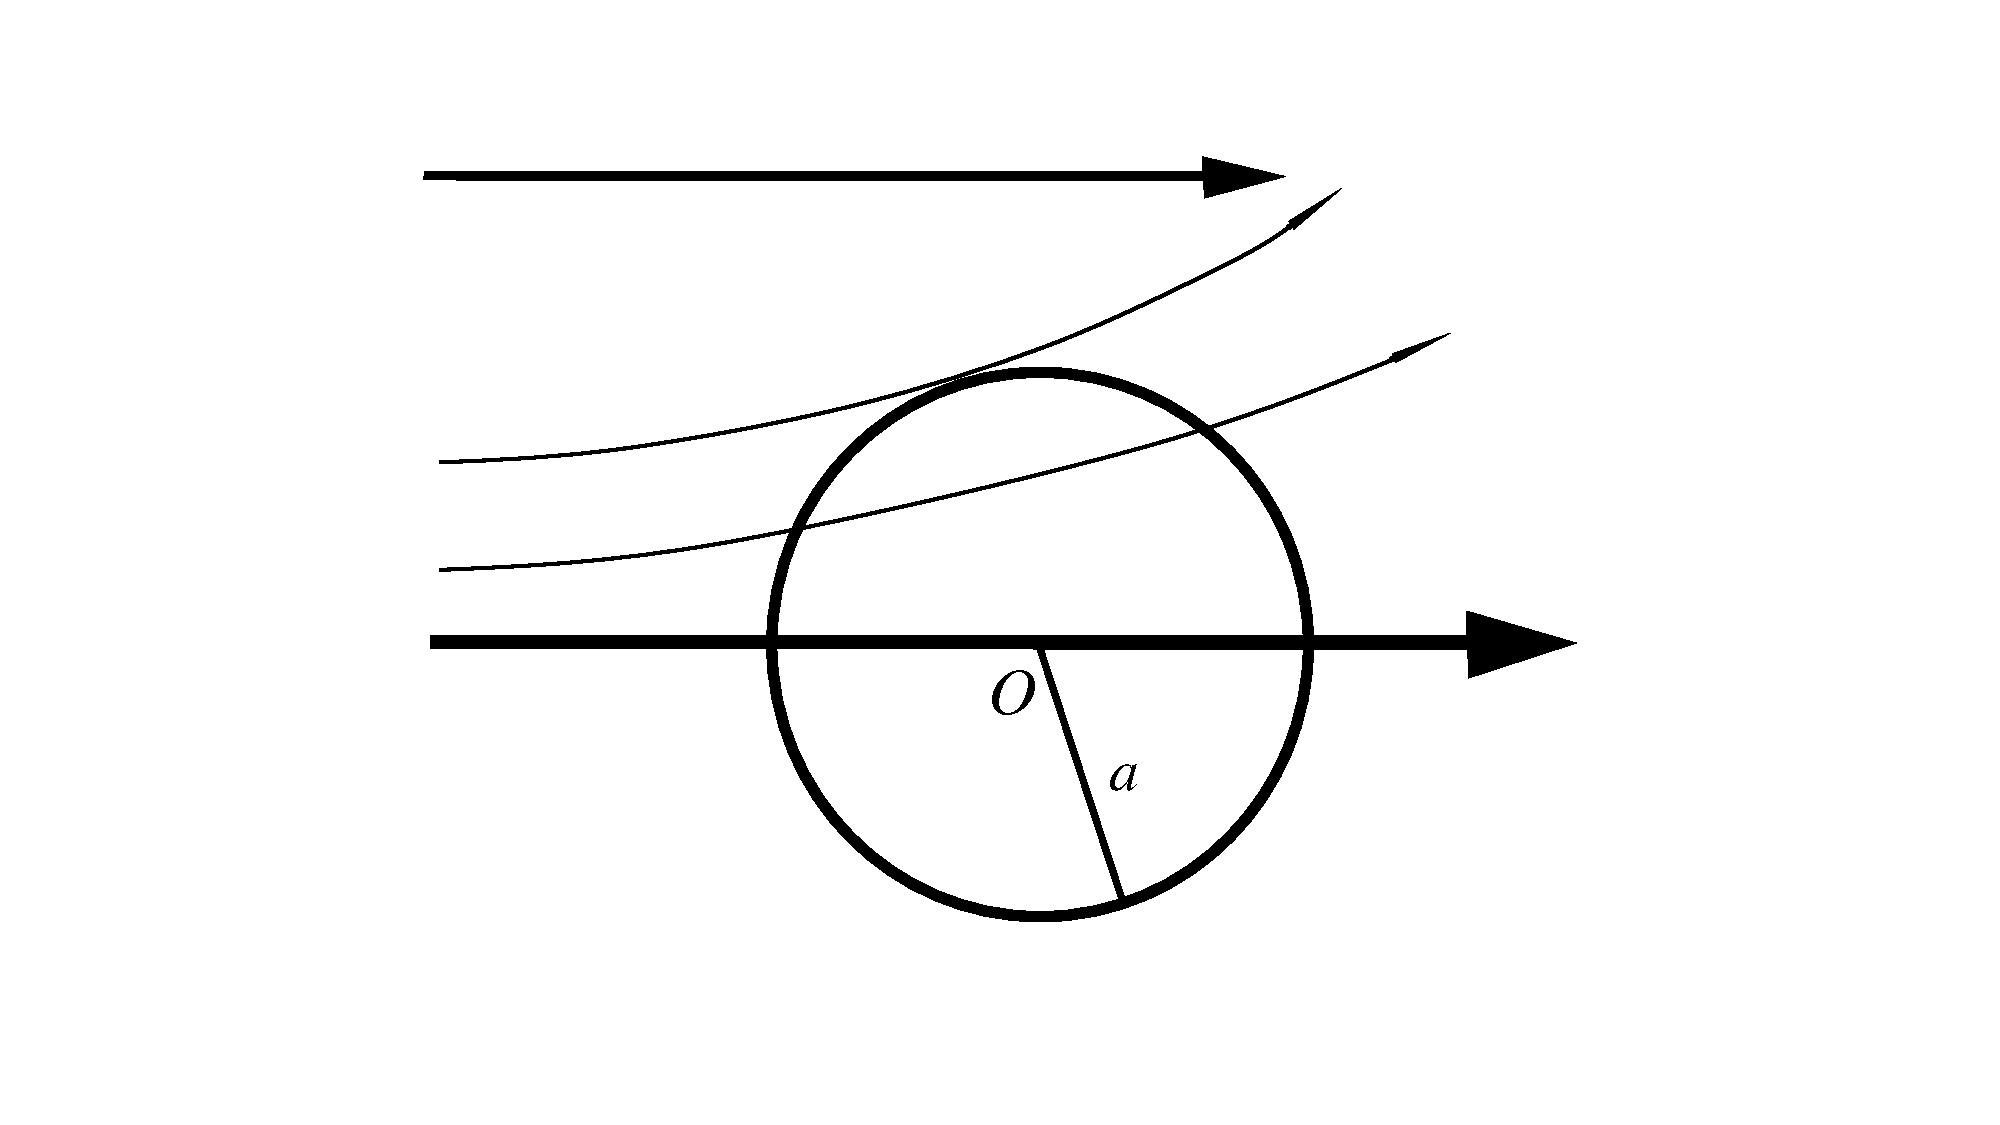
\includegraphics[width=2.5cm,clip]{QM file/figure/1-5}
	\caption{}
	\label{fig.1-5}
\end{wrapfigure}
令一束$\alpha$粒子以相同的初速度$v_{o}$射向一个汤姆孙原子,原子的正电荷($Q=Ze$,Z为原子序数)以库仑力作用于$\alpha$粒子,力的横向分量使$\alpha$粒子运动方向发生偏转.显然,在正电荷边缘掠过的$\alpha$粒子受到的横向力最大,偏转角也最大,如\ref{fig.1-5}所示.下面估算一下最大偏转角的量级.最大横向力约为
\begin{equation*}
	F_{\perp}\sim 2\e\cdot\frac{Z\e}{a^{2}}
\end{equation*}
有效作用时间约为$t\sim\frac{2a}{v_{0}}$,由此获得的横向动量约为
\begin{equation*}
	p_{\perp}\sim F_{\perp}\cdot t \sim\frac{4Z\e^{2}}{av_{0}}
\end{equation*}
因此,最大偏转角约为
\begin{equation}\label{eqn:01.03.07}
	\theta_{max}\sim \frac{p_{\perp}}{m_{a}v_{0}}\sim\frac{4Z\e^{2}}{m_{a}v_{0}^{2}a}=\frac{2Z\e^{2}/a}{E}
\end{equation}
其中$E=\frac{1}{2}m_{a}v_{0}^{2}$是$\alpha$粒子入射动能,$\frac{2Z\e^{2}}{a}$是最大静电势能.

以$\alpha$粒子被金原子(Z=79)散射为例,如取$a\sim 0.1\si{nm}$,$E\sim 5\si{MeV}$,则
\begin{gather}
	\frac{2Z\e^{2}}{a}\sim 2.3\times10^{-3} \si{MeV} \notag \\
	\theta_{max}\sim 4.6\times10^{-4} \notag
\end{gather}
而实验发现,最大偏转角可以超过$\frac{\pi}{2}$,甚至接近$\pi$.对实验结果的统计分析表明,这种大偏转角绝非多次散射的结果,而是由单次散射造成的.由此可知,原子中正电荷的分布半径应该远小于原子半径.为了解释大偏转角散射,原子中正电荷分布半径$R_{0}$应该满足关系:
\setlength{\mathindent}{12em}
\begin{equation}\label{eqn:01.03.08}
	\frac{2Z\e^{2}}{R_{0}} > E
\end{equation}
\eqnormal
这样,当$\alpha$粒子到达正电荷附近某个大于$R_{0}$的距离r时,静电势能$\frac{2Z\e^{2}}{r}$已经接近总能E,速度变小,在横向作用力的推动下,将形成大偏转角.如仍取Z=79,$E=5\si{MeV}$,\eqref{eqn:01.03.08}式给出$R<4.6\times10^{-14}\si{m}$,其量级稍大于原子核半径.

1912年,卢瑟福分析了$\alpha$粒子散射的实验结果后,提出了一种类似于太阳系的原子结构模型,即原子有核模型:原子的正电荷及绝大部分质量集中在很小的原子核(半径不超过10\si{fm})中,形成原子的坚实核心.电子在原子核的库仑力吸引下,环绕原子核运动,电子的轨道半径即原子半径.

在电磁辐射问题上,卢瑟福原子模型遭到了严重的困难,其程度较之汤姆孙模型有过之而无不及.按照经典力学,在原子核的库仑力场作用下,电子可以沿圆形或椭圆形轨道运动,原子核位于轨道的焦点处.电子运动的总机械能为负,并与圆的半径或椭圆的长半径成反比$\bigg(E=-\frac{Z\e^{2}}{2a} \bigg)$.按照经典电动力学,带电质点作加速运动时,将辐射电磁波.因此电子在运动过程中,将不断辐射电磁波,即发光,其频率等于电子的轨道频率及其倍频.由于对外辐射电磁波,电子运动的总能逐渐降低,轨道半径逐渐缩小,而运转频率则逐渐加快($\nu\propto a^{\frac{-3}{2}}$),最后电子将落入原子核中,即原子将崩溃.按照经典力学和电动力学的计算,如取初始原子半径$a\sim 0.1\si{nm}$,由于电磁辐射而造成原子崩溃的时间约为$10^{-10}\si{s}$.在此过程中,电子将辐射出各种频率的电磁波,频率呈现连续分布.

以上就是按照卢瑟福原子模型和经典物理理论描绘的原子辐射的情景,它显然与光谱公式\eqref{eqn:01.03.02}不符合,也与原子可以稳定存在这样一个经过多次实验证实的事实有着根本矛盾.

\textsf{3. 玻尔的量子论}

1913年,年仅28随的丹麦物理学家玻尔(N.Bohr)提出了原子结构的量子论.玻尔将卢瑟福原子模型和普朗克-爱因斯坦关于光辐射的量子论结合起来,扬弃了经典物理学的某些基本概念,而代之以一系列的量子假设.玻尔量子论的要点如下:

(1) 玻尔承认卢瑟福原子模型,但认为原子中的电子只能处于某些具有特定能量的状态(稳定轨道).如果没有外界作用,电子将始终沿着同一条稳定轨道运动,不辐射电磁波.也就是说,玻尔假定,对于电子的这些稳定状态,电动力学规律失效.

(2) 在外界作用下,如电子从一个稳定状态跃迁到另一个能量较低的稳定状态,则在此状态跃迁过程中,电子将发光(辐射电磁波),其频率为
\eqshort
\begin{equation}\label{eqn:01.03.09}
	\nu=\frac{E_{n}-E_{n^{\prime}}}{h}
\end{equation}\eqnormal
上式称为频率规则,$h$为普朗克常量.容易理解,\eqref{eqn:01.03.09}式是能量守恒定律和光量子概念的必然结论,但它与经典电动力学二理论存在根本概念上的矛盾.按照电动力学,电磁辐射频率应该等于电子当时的轨道运转频率,而\eqref{eqn:01.03.09}式则由跃迁前后两个状态的能量差决定.

(3) 在经典力学所允许的各个轨道中,只有符合量子化条件的轨道才是稳定轨道.玻尔当时只考虑了圆形轨道,提出的量子化条件为:轨道角动量的取值必须等于$h$(即$h/2\pi$)的整数倍,即
\begin{equation}\label{eqn:01.03.10}
	L=m_{e}vr=n\hbar,\quad n=1,2,3,\cdots
\end{equation}\eqlong
玻尔利用量子化条件\eqref{eqn:01.03.10}和频率规则\eqref{eqn:01.03.09},求出了氢原子中电子的稳定轨道的半径和能量,以及光谱频率,成功地解释了氢原子光谱公式\eqref{eqn:01.03.02}.

\begin{wrapfigure}[7]{r}{6em}
	\centering
	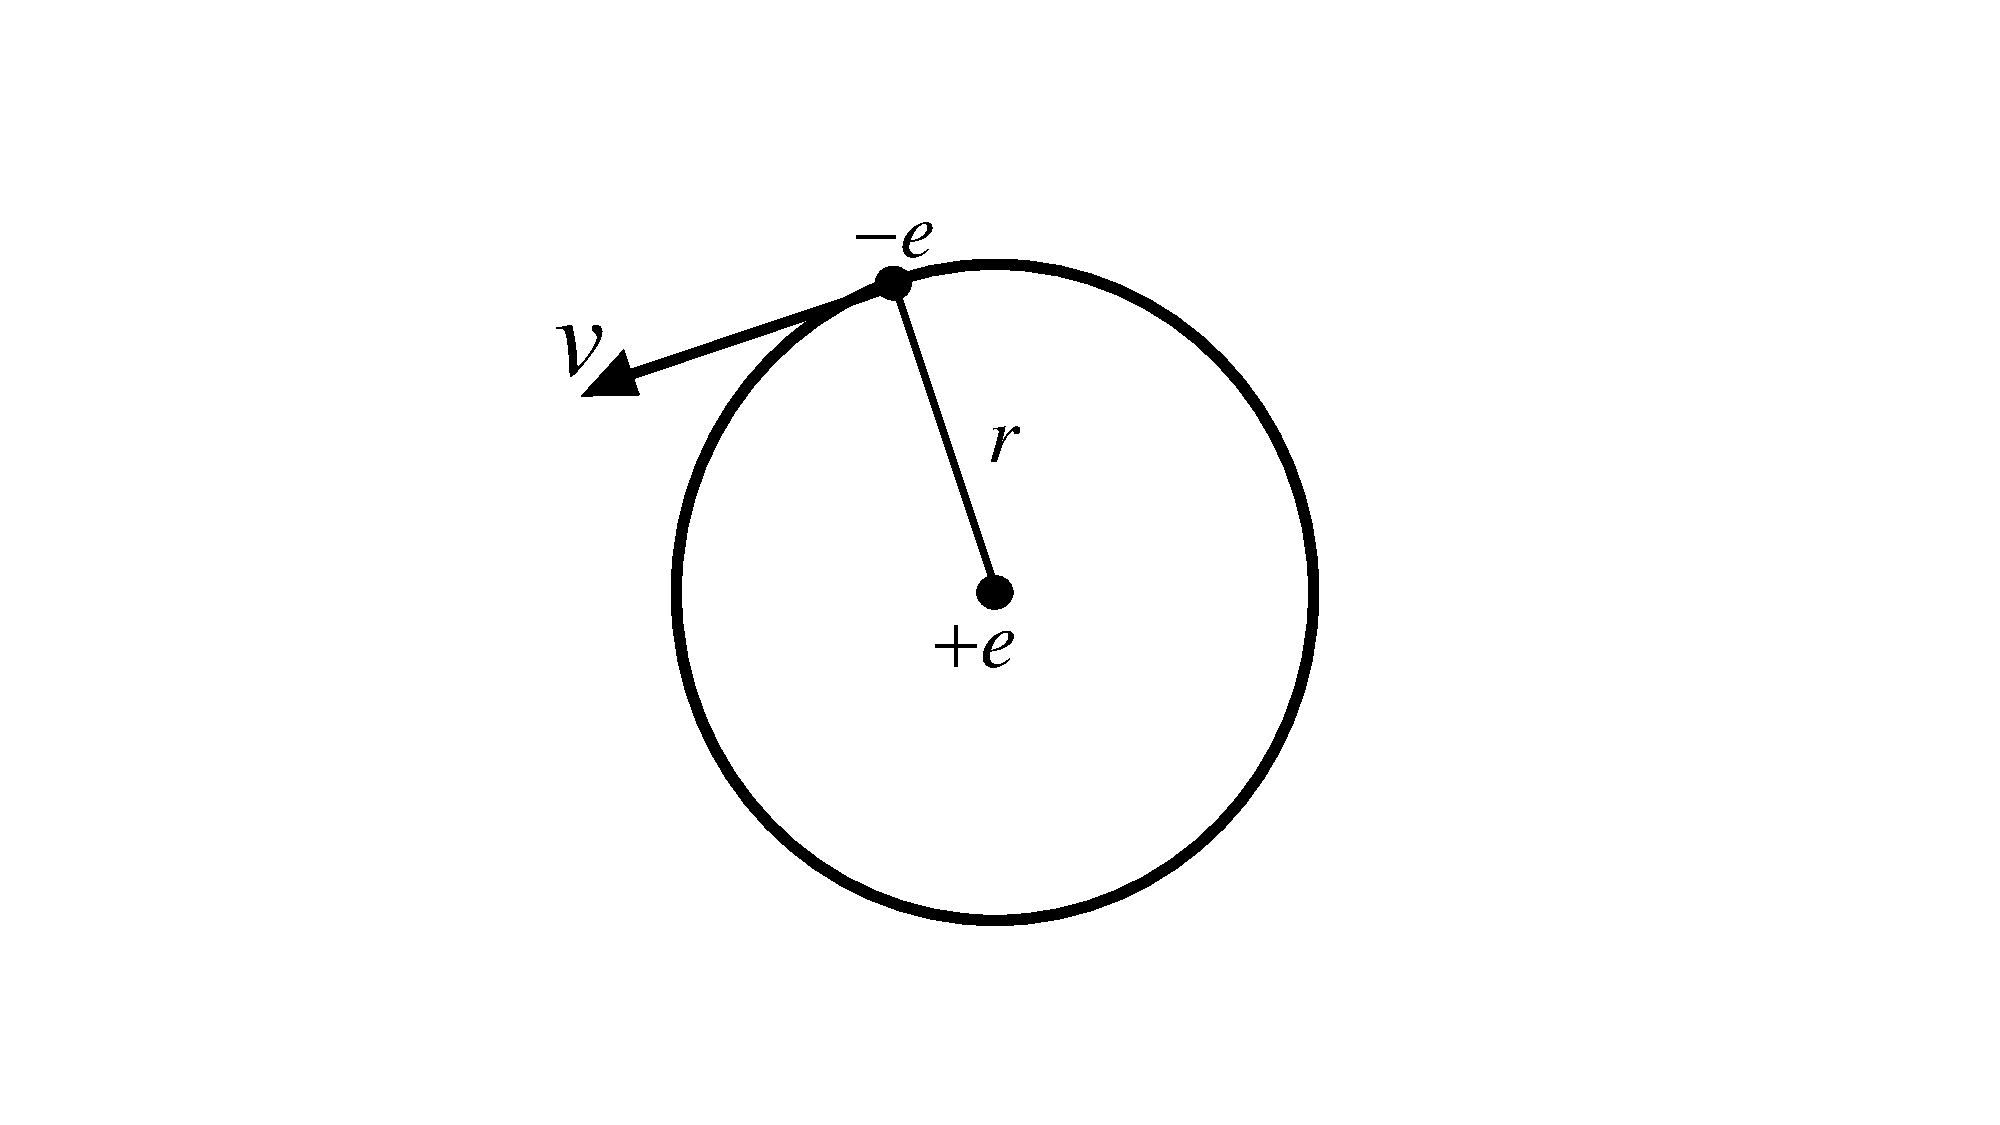
\includegraphics[width=2cm,clip]{QM file/figure/1-6}
	\caption{}
	\label{fig.1-6}
\end{wrapfigure}
后来,索末菲(Sommerfeld)将玻尔地量子化条件推广成为
\begin{equation}\label{eqn:01.03.11}
	\oint pdq =nh\quad n=1,2,3,\cdots
\end{equation}\eqshort
$p,q$为一对共轭地正则动量和坐标,$\oint$表示对运动的一个周期积分.推广后的量子化条件可以适用于任何周期性轨道,例如氢原子中电子的椭圆轨道.

玻尔认为,量子理论和经典物理理论之间并无不可逾越的鸿沟.量子理论概念适用于微观尺度,也适用于宏观尺度,经典理论仅适用于宏观尺度,在宏观尺度上,两种理论应该是一致的.这个观点成为对应原理.玻尔在20世纪20年代到各国宣讲他的量子理论时,强调对应原理是一个核心概念,而量子化条件则并不重要.下面我们根据对应原理对氢原子的能级和光谱试作分析.

考虑到圆轨道\ref{fig.1-6},电子的轨道半径r,速率v和角频率(角速度)$\omega$间的关系是
\begin{equation}\label{eqn:01.03.12}
	v=r\omega
\end{equation}
\eqnormal
原子核(电荷e)对电子的库伦吸引力就是圆周运动的向心力,
\begin{equation*}
	\frac{\e^{2}}{r^{2}}=m_{e}\frac{v^{2}}{r}=m_{e}r\omega^{2}
\end{equation*}\eqshort
因此
\begin{equation}\label{eqn:01.03.13}
	r^{3}\omega^{2}=\frac{\e^{2}}{m_{e}}
\end{equation}\eqnormal
电子运动的总能为
\begin{equation*}
	E=\frac{1}{2}m_{e}v^{2}-\frac{\e^{2}}{r}=\frac{1}{2}m_{e}r^{2}\omega^{2}-\frac{\e^{2}}{r}
\end{equation*}\eqshort
利用\eqref{eqn:01.03.13}式,得到
\begin{equation}\label{eqn:01.03.14}
	E=-\frac{\e^{2}}{2r}
\end{equation}\eqnormal
或
\begin{equation}\label{eqn:01.03.15}
	\omega=\bigg(\frac{8}{m_{e} \e^{4}}\bigg)^{\frac{1}{2}}(-E)^{\frac{3}{2}}
\end{equation}
\eqref{eqn:01.03.13}至\eqref{eqn:01.03.13}式适用于任何一条圆形轨道.以$n=1,2,3,\cdots$表示稳定轨道的序号,相应的$r,E,\omega$记为$r_{n},E_{n},\omega_{n}$,并规定$r_{n}$的编号次序为$r_1 < r_2 < r_3<\cdots$,当n不断增大,$r_{n}\rightarrow\infty$,$E_{n}\rightarrow 0^{-}$,所以$n\gg 1$相当于宏观尺度.

当电子由能级$E_{n}$跃迁到$E_{n-1}$,按照频率规则,发光角频率为
\begin{equation}\label{eqn:01.03.16}
	\omega=2\pi v=\frac{E_{n}-E_{n-1}}{\hbar}
\end{equation}
而按照电动力学,发光频率等于轨道运转频率,即$\omega_{n}$.按照对应原理,在$n\gg 1$时,$\omega$应该趋于$\omega_{n}$,即
\begin{equation}\label{eqn:01.03.17}
	E_{n}- E_{n-1}=\hbar\omega\rightarrow\hbar\omega_{n}
\end{equation}
亦即
\begin{equation}\label{eqn:01.03.18}
	E_{n}- E_{n-1}\rightarrow \bigg(\frac{8\hbar^{2}}{m_{e}\e^{4}}\bigg)^{\frac{1}{2}} (-E_{n})^{\frac{3}{2}},\quad n\gg 1
\end{equation}
$n\gg 1$时,n的变化($\Delta n=1$)远小于n本身,可以当作连续变化,因此
\begin{equation*}
	E_{n}- E_{n-1}=\Delta E_{n}
	=\frac{\Delta E_{n}}{\Delta n}\rightarrow\frac{dE_{n}}{dn}
\end{equation*}
\eqref{eqn:01.03.18}式可当作微分方程:
\begin{equation*}\label{eqn:01.03.18'}
	 \frac{dE_{n}}{dn}=
	 \bigg(\frac{8\hbar^{2}}{m_{e}\e^{4}}\bigg)^{\frac{1}{2}}(-E_{n})^{\frac{3}{2}},
	 \quad n\gg1		\tag{$1.3.18^{\prime}$}
\end{equation*}
容易解出
\begin{equation}\label{eqn:01.03.19}
	E_{n}=-\frac{1}{2n^{2}}\frac{m_{e}\e^{4}}{\hbar^{2}}=-\frac{1}{2n^{2}}\frac{\e^{2}}{a_{0}}
\end{equation}
再利用\eqref{eqn:01.03.14}式,得到
\begin{equation}\label{eqn:01.03.20}
	r_{n}=-\frac{\e^{2}}{2E_{n}}=n^{2}\frac{\hbar^{2}}{m_{e}\e^{2}}=n^{2}a_{0}
\end{equation}
其中$a_{o}=\frac{\hbar^{2}}{m_{e}\e^{2}}$为玻尔半径,即氢原子基态(n=1)半径.\eqref{eqn:01.03.19}、\eqref{eqn:01.03.20}式是在条件$n\gg 1$下得到的,如果认为这些结果也适用于n较小的情况,则它们就是氢原子能级和轨道半径的量子化公式.

以L表示轨道角动量,利用\eqref{eqn:01.03.13}及\eqref{eqn:01.03.20}式,容易得到
\begin{equation*}
	L^{2}=(m_{e}vr^{2})^{2}=m_{e}^{2}\omega^{2}r^{4}=m_{e}^{2}\frac{\e^{2}}{m_{e}}n^{2}\frac{\hbar^{2}}{m_{e}\e^{2}}=n^{2}\hbar^{2}
\end{equation*}
亦即
\begin{equation*}
	L=n\hbar,\quad n=1,2,3,\cdots
\end{equation*}
这正是量子化条件\eqref{eqn:01.03.10}.

当电子由能级跃迁但,按照频率规则\eqref{eqn:01.03.09},放光频率为
\begin{equation}\label{eqn:01.03.21}
	\nu_{nm}=\frac{E_{n}-E_{m}}{h}=2\pi^{2}\frac{m_{e}\e^{4}}{h^{3}}\bigg(\frac{1}{m^{2}} -\frac{1}{n^{2}}\bigg)
\end{equation}
和经验公式\eqref{eqn:01.03.02}比较,二者一致,并得里德伯(Rydberg)常数的结构式:
\begin{equation}\label{eqn:01.03.22}
	R=\frac{2\pi^{2}m_{e}\e^{4}}{ch^{3}}=\frac{m_{e}\e^{4}}{4\pi c\hbar^{3}}
\end{equation}
以各基本常数之值代入上式,得到R的理论值为$R=\num{109737}\si{cm^{-1}}$.严格地说,氢原子问题是二体问题,求电子能级时应该用折合质量$\mu=\frac{m_{e}m_{p}}{m_{e}+m_{p}}$代替以上计算中地电子质量$m_{e}$,这样得到的氢原子光谱里德伯常数理论值为
\begin{equation}\label{eqn:01.03.23}
	R_{H}=\frac{2\pi^{2}\mu \e^{4}}{ch^{3}}=\num{109677} \si{cm^{-1}}
\end{equation}
和实验值符合得极好.

\example 对于氢原子的第n个玻尔圆形轨道,求电子运行速度.

\solution 根据量子化条件\eqref{eqn:01.03.10}及轨道半径公式\eqref{eqn:01.03.20},易得速度公式:
\begin{equation*}
	v=\frac{n\hbar}{m_{e}r_{n}}=\frac{\hbar}{nm_{e}a_{0}}=\frac{\e^{2}}{n\hbar}=\frac{c}{n}\frac{\e^{2}}{\hbar c}
\end{equation*}\eqshort
其中$\frac{\e^{2}}{\hbar c}=\frac{1}{137}$,所以
\begin{equation}\label{eqn:01.03.24}
	v=\frac{c}{137}\cdot\frac{1}{n}
\end{equation}\eqnormal
按数量级而言,$v$约为光速的几百分之一,约为$10^{6}\si{m/s}$.


% 原子物理中的特征量
\section[原子物理中的特征量]{原子物理中的特征量}\label{sec:01.04}
% \makebox[5em][s]{} % 短题目拉间距
% \setlength{\mathindent}{9em} 本文标准公式缩进 
% \eqnormal % 恢复标准缩进


微观现象得普遍特点之一就是“量子化”,表征问题的各主要物理量常有一定的量级,它们和各个基本常数(常量)常有一定的构造关系.这种构造关系常可根据某些判据,利用量纲方法予以导出.

\textsf{1. 基本常数}

基本普适常数通常总是与某种基本物理规律相联系,例如玻耳兹曼常数K代表热平衡下的统计规律,光速c 表示相对论效应和电磁定律, 普朗克常数$\hbar$代表量子理论,元电荷e是电荷的量子化单位,等等.基本普适常数没有结构可言,它们表征着当今人类对客观物质世界的认识水平,它们的数值直接由实验决定.当问题涉及到某种基本粒子(例如电子)时,粒子的质量和自旋也是基本常数.
$\bigg($自旋总是$\hbar$的$\frac{n}{2}$倍,$n=0,1,2,\cdots$,通常可以不必另行作为基本常数提出. $\bigg)$

由于库仑定律的表现形式为$F=-\frac{e_{1}e_{2}}{r^{2}}$,所以$e^{2}$具有(能量)$\times$(长度)的量纲,和$\hbar c$的量纲相同,因此$\frac{e^{2}}{\hbar c}$是无量纲普适常数,它表征着基本电荷间的电磁作用.历史上它是在研究原子光谱的精细结构时被发现的,故称精细结构常数,其数值为
\begin{equation*}
	\frac{\e}{\hbar c}\bigg(\text{即}\frac{1}{4\pi\varepsilon_{0}}\frac{e}{\hbar c} \bigg)=\num{7.29335}\times10^{-3} \approx \frac{1}{137}
\end{equation*}
这是一个十分重要的普适常数,有些量纲相同的特征量之间的相互关系常可通过精细结构常数表示出来.

\textsf{2. 原子能级}

电子的相对论静能为$m_{e}c^{2}=0.51 \si{MeV}$.研究电子运动时,如果能量变化远小于$m_{e}c^{2}$,为低速运动,这时原则上可以不用相对论理论.如能量的变化接近或超过$m_{e}c^{2}$,为高速运动,即高能范围,必须用相对论理论.

根据实验测定,原子的(外层)电子能级,量级约10 \si{eV}, 远小于$m_{e}c^{2}$,属于非相对论范围.由于电荷间的库仑力也与c无关,所以可以断定原子的电子能级公式中不会出现光速c.利用这个判据, 易知电子能级的特征值(不包括静能$m_{e}c^{2}$)必为
\begin{equation}\label{eq14.1}
	\begin{aligned}
		E &\sim m_{e}c^{2}\bigg(\frac{\e}{\hbar c} \bigg)^{2}= \frac{m_{e}e^{4}}{\hbar^{2}} \\
		&\sim \num{0.511}\times10^{6}\si{eV}\times\bigg(\frac{1}{137} \bigg)^{2}\sim \num{27.2}\si{eV}
	\end{aligned}
\end{equation}\eqshort

\textsf{3. 特征长度}

上述电子能级特征值可以写成
\begin{equation}\label{eq14.2}
	E\sim \frac{\e^{2}}{a_{0}}
\end{equation}\eqnormal
其中
\begin{equation}\label{eq14.3}
	a_{0}=\frac{\hbar^{2}}{m_{e}\e^{2}}-\num{0.53}\times 10^{-10}\si{m}
\end{equation}\eqshort
是原子结构的特征长度,即玻尔半径.它是量子论的(含有$\hbar$),又是非相对论的(与c无关).

原子光谱的波长$\lambda=\frac{c}{\nu}$,$\nu$为频率.根据玻尔量子论[见\eqref{eqn:01.03.09}式],$\nu=\frac{E_{n}-E_{n^{\prime}}}{h}$所以
\begin{equation}\label{eq14.4}
	\lambda=\frac{hc}{E_{n}-E_{n^{\prime}}}
\end{equation}
能级差($E_{n}-E_{n^{\prime}}$)一般为几个\si{eV},而hc的值为
\begin{equation*}
	hc=1.24\times10^{-6} \si{eV\cdot m}
\end{equation*}\eqlong
所以$\lambda$一般为$10^{2}\sim10^{3} \si{nm}$量级.例如当($E_{n}-E_{n^{\prime}}$)= =2 \si{eV},$\lambda$=620 \si{nm} ,属于可见光范围.

玻尔半径$a_{0}$和精细结构常数相乘,即得电子的约化康普顿波长:
\begin{equation}\label{eq14.5}
	\lambdabar_{c}=a_{0}\bigg(\frac{\e}{\hbar c} \bigg)=\frac{\hbar}{m_{e}c}\sim\frac{a_{0}}{137}\sim3.86\times10^{-13}\si{m}
\end{equation}\eqnormal
原始的康普顿波长(见\ref{sec:01.02})是指
\begin{equation}\label{eq14.6}
	\lambda_{c}=\frac{h}{m_{e}c}\sim2.43\times10^{-12} \si{m}
\end{equation}
康普顿波长与$h,c$及粒子质量有关(但与电荷无关),故凡相对论和量子论同时起决定性作用的现象中,特征长度通常就是康普顿波长.例如(电子、正电子)对的产生或湮没,就在康普顿波长的范围内发生. 又如核力(强作用)的传递是与$\pi$介子的产生和湮没相联系的,但与电磁作用无关,因此核力的力程必为$\pi$介子的康普顿波长的量级,即
\begin{equation}\label{eq14.7}
	\text{核力力程} \sim\frac{\hbar}{m_{\pi}c} \sim\frac{\lambdabar_{c}}{270}\sim 1.4\si{fm}
\end{equation}
($m_{\pi}\sim 270 m_{e}$),这与核力力程的公认实验值(约2 \si{fm}左右)是一致的.

有关电子运动的另一个更小的特征长度是电子经典半径:
\begin{equation}\label{eq14.8}
	r_{e}=\lambdabar_{e}\bigg(\frac{\e}{\hbar c} \bigg)=\frac{\e^{2}}{m_{e}c^2}\sim 2.8 \si{fm}
\end{equation}
它与量子论无关(与h 无关),故称“经典半径”.其实电子的真实“半径”远小于$10^{3} \si{fm}$. 现今在前沿理论中,电子通常当作点电荷对待.

\textsf{4. 速度和角速度}

原子中电子的运动属于低能范围,电子速度v的公式应该与c无关,因此可以断定
\begin{equation}\label{eq14.9}
	v\sim c \cdot\frac{\e}{\hbar c}=\frac{\e^{2}}{\hbar}\sim\frac{c}{137}
\end{equation}
也可以利用能级特征值公式\eqref{eq14.1},并利用$E\sim m_{e}v^{2}$得出\eqref{eq14.9}式.上式大致表征了外层电子(价电子)的速度.在原子的最内层,电子所受作用力大体上就是直接来自原子核(电荷$Ze$,$Z$为原子序数)的未经其他电子屏蔽的库仑力,$F\sim\frac{Z\e^{2}}{r^{2}}$,这时\eqref{eq14.1}式和\eqref{eq14.9}式中$\e^{2}$应换成$Z\e^{2}$,因此$v\sim\frac{cZ}{137}$,当Z较大时,v可达光速c的一半以上.这种情况下应该用相对论量子力学来描写电子的运动.

电子沿基态玻尔轨道(n = 1)运动时,角速度为
\begin{equation}\label{eq14.10}
	\omega_{1}=\frac{v}{a}\sim\frac{1}{137}\frac{c}{a_{0}}4.1\times10^{16} \si{s^{-1}}
\end{equation}\eqshort
沿量子数为n的圆轨道运动时,由$\S$\ref{sec:01.03}\eqref{eqn:01.03.13},\eqref{eqn:01.03.20}式,可得角速度为
\begin{equation}\label{eq14.11}
	\omega_{n}=\frac{\omega_{1}}{n^{3}}
\end{equation}\eqnormal
电子的轨道周期为$\frac{2\pi}{\omega}$,对于第n个玻尔圆轨道,周期为
\begin{equation}\label{eq14.12}
	\frac{2\pi}{\omega_{n}}=n^{3}\frac{2\pi}{\omega_{1}}=\frac{2\pi n^{3}\hbar^{3}}{m_{e}\e^{4}}
\end{equation}\eqlong
其中
\begin{equation}\label{eq14.13}
	\frac{2\pi}{\omega_{1}}=2\pi\frac{\hbar}{m_{e}\e^{4}}=2\pi\times137\frac{a_{0}}{c}\sim1.5\times10^{-16} \si{s}
\end{equation}\eqnormal

\textsf{5. 电矩和磁矩}

原子的内层电子大致呈球对称分布,对电矩和磁矩无贡献,原子的电矩和磁矩主要来自外层电子.以氢原子为例,电偶极矩约为
\begin{equation}\label{eq14.14}
	D\sim er\sim ea_{0}=\frac{\hbar^{2}}{m_{e}\e}\quad(n=1)
\end{equation}

电子沿圆形轨道匀速运动时,相当于一个环形电流,环的面积为$A=\pi r^{3}$,电流为$I=-\frac{\e\omega}{2\pi}$.按照电磁理论,这种环形电流的等效磁矩为
\begin{equation}\label{eq14.15}
	\begin{aligned}
		\mu=IA=-\frac{\e r^{2}\omega}{2} \text{(国际单位制)} \\
		\mu=\frac{IA}{c}=-\frac{\e r^{2}\omega}{2c} \text{(高斯单位制)}
	\end{aligned}
\end{equation}
电子的轨道角动量为$L=m_{e}vr=m_{e}r^{2}\omega$,所以磁矩和角动量的关系为
\begin{equation}\label{eq14.16}
	\begin{aligned}
		\boldsymbol{\mu}&=-\frac{\e}{2m_{e}}\boldsymbol{L} \text{(国际单位制)} \\
		\boldsymbol{\mu}&=-\frac{\e}{2m_{e}c}\boldsymbol{L} \text{(高斯单位制)}
	\end{aligned}
\end{equation}
由于电子电荷为负,轨道角动量$\boldsymbol{L}$的方向和磁矩$\mu$的方向相反.容易证明,\eqref{eq14.16}式也适用于椭圆轨道.按照玻尔的量子化条件,角动量L 是量子化的,其单元为$\hbar$,因此磁矩$\mu$也是量子化的,其单元为“玻尔磁子”:
\begin{equation}\label{eq14.17}
	\begin{aligned}
		\mu_{B}&=-\frac{\e\hbar}{2m_{e}} \text{(国际单位制)} \\
		\mu_{B}&=-\frac{\e\hbar}{2m_{e}c} \text{(高斯单位制)}
	\end{aligned}
\end{equation}\eqshort
国际单位制中,电矩与磁矩量纲不同在高斯单位制中,电矩与磁矩量纲相同,比值约为
\begin{equation}\label{eq14.18}
	\frac{\mu}{D}\sim\frac{\e^{2}}{\hbar c}\sim\frac{1}{137}
\end{equation}

\textsf{6. 经典电偶极矩振子的辐射功率}

具有确定频率$\nu=\frac{\omega}{2\pi}$的电偶极矩振子,其电偶极矩为
\begin{equation}\label{eq14.19}
	D(t)=D\cos\omega t
\end{equation}
按照经典电动力学理论,这个偶极矩振子将向外辐射同样频率的电磁波,总辐射功率为
\begin{equation}\label{eq14.20}
	-\frac{dE}{dt}=\frac{D^{2}\omega^{4}}{3c^{3}}
\end{equation}
电子以角速度$\omega$沿半径为r的圆周运动时,相当于两个振动方向互相垂直的电偶极矩振子($D = er$),按照电动力学,其总辐射功率为
\begin{equation}\label{eq14.21}
	-\frac{dE}{dt}=\frac{2}{3}\frac{\e^{2}r^{2}\omega^{4}}{c^{3}}
\end{equation}\eqnormal
在这里我们用虽纲方法对这两个公式作一些说明.如果偶极振子确实存在电磁辐射,其总辐射功率显然取决于电偶极矩振幅D,角频率$\omega$以及光速c(来自麦克斯韦方程).它们的量纲为
\begin{gather} 
	c—— \si{LT^{-1}},\quad \omega—— \si{T^{-1}},\quad \frac{c}{\omega}—— \si{L} \notag\\
	\frac{dE}{dt}—— \si{ET^{-1}}.\quad D^{2}—— \e^{2}r^{2}—— \si{EL^{3}} \notag
\end{gather}\eqshort
因此,辐射功率唯一可能的量纲构造方式为
\begin{equation}\label{eq14.22}
	-\frac{dE}{dt}\sim\frac{D^{2}\omega^{4}}{c^{3}}
\end{equation}\eqnormal
它和电动力学的严格计算结果\eqref{eq14.20}、\eqref{eq14.21}式只相差一个量级为1的纯数值系数.

\textsf{7. 原子激发态的平均寿命}

按照玻尔量子论,原子中的电子停留在某个能级(稳定轨道)上时,并不辐射电磁波;当电子由某个较高能级跃迁到较低能级时,将辐射电磁波(光子).实验发现,对于一个原子,这种能级跃迁是突变式的, 但带有概率性,大最处于相同能级的原子,它们的能级跃迁并非同时发生,而是大体上在某段时间$\tau$内完成,$\tau$称为初始能级的平均寿命.利用对应原理分析能级跃迁过程得到的结论是,原子能级跃迁过程的电磁辐射性质,相当于经典电偶极矩振子.以氢原子中电子由能级$E_{2}$跃迁到$E_{1}$为例,跃迁过程释放出的总能量为($E_{2}-E_{1}$),辐射角频率为$\omega=\frac{E_{2}-E_{1}}{\hbar}$,相应的电偶极矩振幅可以估计为$\sim ea_{0}$,因此辐射功率约为
\begin{equation*}
	-\frac{dE}{dt}\sim\frac{D^{2}\omega^{4}}{c^{3}}\sim
	\frac{\e^{2}a_{0}^{2}(E_{2}-E_{1})^{4}}{c^{3}\hbar^{4}}
\end{equation*}
因此电子停留在激发态能级($E_{2}$)的平均寿命约为
\begin{equation}\label{eq14.23}
	\tau\sim\frac{E_{2}-E_{1}}{|\frac{dE}{dt}|}\sim
	\frac{c^{3}\hbar^{4}}{\e^{2}a_{0}^{2}(E_{2}-E_{1})^{3}}
\end{equation}
由$\S$\ref{sec:01.03}\eqref{eqn:01.03.19}式
\begin{equation*}
	E_{2}-E_{1}=\frac{3}{8}\frac{\e^{2}}{a_{0}}=\frac{3}{8}\frac{m_{e}\e^{4}}{\hbar^{2}}\sim10.2\si{eV}
\end{equation*}
代入\eqref{eq14.23}式,得到
\eqlong
\begin{equation}\label{eq14.24}
	\begin{aligned}
		\tau &\sim \bigg(\frac{8}{3} \bigg)^{3} \bigg(\frac{\hbar c}{\e^{2}} \bigg)^{4} \frac{a_{0}}{c}  \\
		&\sim \bigg(\frac{8}{3} \bigg)^{3} (137)^{4} \frac{0.53\times10^{-10}}{3\times10^{8}}\si{s} \approx1.2\times10^{-9}\si{s}
	\end{aligned}
\end{equation}
扯子力学的精确计算结果为(见$\S 9.4$)%(见$\S$\ref{sec:09.04})
\begin{equation}\label{eq14.25}
	\tau_{2p\rightarrow 1s}=
	\bigg(\frac{3}{2} \bigg)^{8} \bigg(\frac{\hbar c}{\e^{2}} \bigg)^{4} \frac{a_{0}}{c}=1.6\times10^{-9} \si{s}
\end{equation}\eqnormal
注意,电子在$E_{2}$能级上的轨道运动周期为[见\eqref{eq14.12}、\eqref{eq14.13}式]
\begin{equation*}
	\frac{2\pi}{\omega_{2}}\sim1.2\times10^{-15} \si{s}
\end{equation*}
处于$E_{2}$轨道上的电子,在跃迁到$E_{1}$轨道之前,在$E_{2}$轨道上的平均运行圈数约为
\begin{equation*}
	\frac{\tau\omega_{2}}{2\pi}\sim \frac{32}{27\pi} \bigg(\frac{\hbar c}{\e^{2}} \bigg)
	\sim 10^{6}
\end{equation*}
“稳定轨道”的意义于此可见一斑.

\eqref{eq14.23}式大致可以适用于其他单价原子的价电子光学跃迁,只是其中$a_{0}$应改为原子半径的实际数值.例如取原子半径$a_{0}\sim0.1 \si{nm}$,当$(E_{2}-E_{1})\sim 2\si{eV}$(发射光波波长$\lambda \sim620 \si{nm}$) ,激发态平均寿命$\tau\sim4.5\times10^{-8}\si{s}$.





% 德布罗意的“物质波”假设
\section[德布罗意的“物质波”假设]{德布罗意的“物质波”假设}\label{sec:01.05}
% \makebox[5em][s]{} % 短题目拉间距
% \setlength{\mathindent}{9em} 本文标准公式缩进 
% \eqnormal % 恢复标准缩进

玻尔量子论的建立,极大地推动了原子物理学的发展.但随着研究的深入,玻尔量子论的局限性也逐渐暴露出来.例如任何一种原子光谱,各条谱线的相对强度表现出很好的规律性,玻尔量子论未能对此作出满意的解释.氨原子光谱表现出某些奇特的规律(似乎是由两套光谱混杂而成),玻尔量子论对此也无力解释长期以来,许多化学和物理理论中,从来认为原子的形状像一个小球,这个概念早已被多种实验事实所肯定. 但在玻尔量子论中,电子作平面轨道运动,因此原子(尤其是氢原子)的形状更像一个饼.

1924年,德布罗意提出了“物质波” 的假设.德布罗意注意到了几何光学(光的宏观传播规律)和质点力学有着惊人的相似性.光在均匀介质中沿直线传播的定律,在两种介质的分界面处光的反射和折射定律,以及在不均匀介质中光沿曲线传播的规律,可以统一为“最小光程原理(费马原理)”, 即
\eqshort
\begin{equation}\label{eq15.1}
	\delta\int_{A}^{B} ndl = 0
\end{equation}\eqnormal
光由A点传播到B点,$\int_{A}^{B}\cdots dl$表示由A到B的线积分,n为折射率,(A,B)间任何一条可能的路径的光程即$\int_{A}^{B}ndl$,光程最小的路径就是实际的光线.牛顿质点力学定律可以表示成“最小作用量原理”,即
\begin{equation}\label{eq15.2}
	\delta\int_{A}^{B}pdl=\delta\int_{A}^{B}\sqrt{2m(E\sim V)}dl
\end{equation}\eqlong
\begin{wrapfigure}[5]{r}{8em}
	\centering
	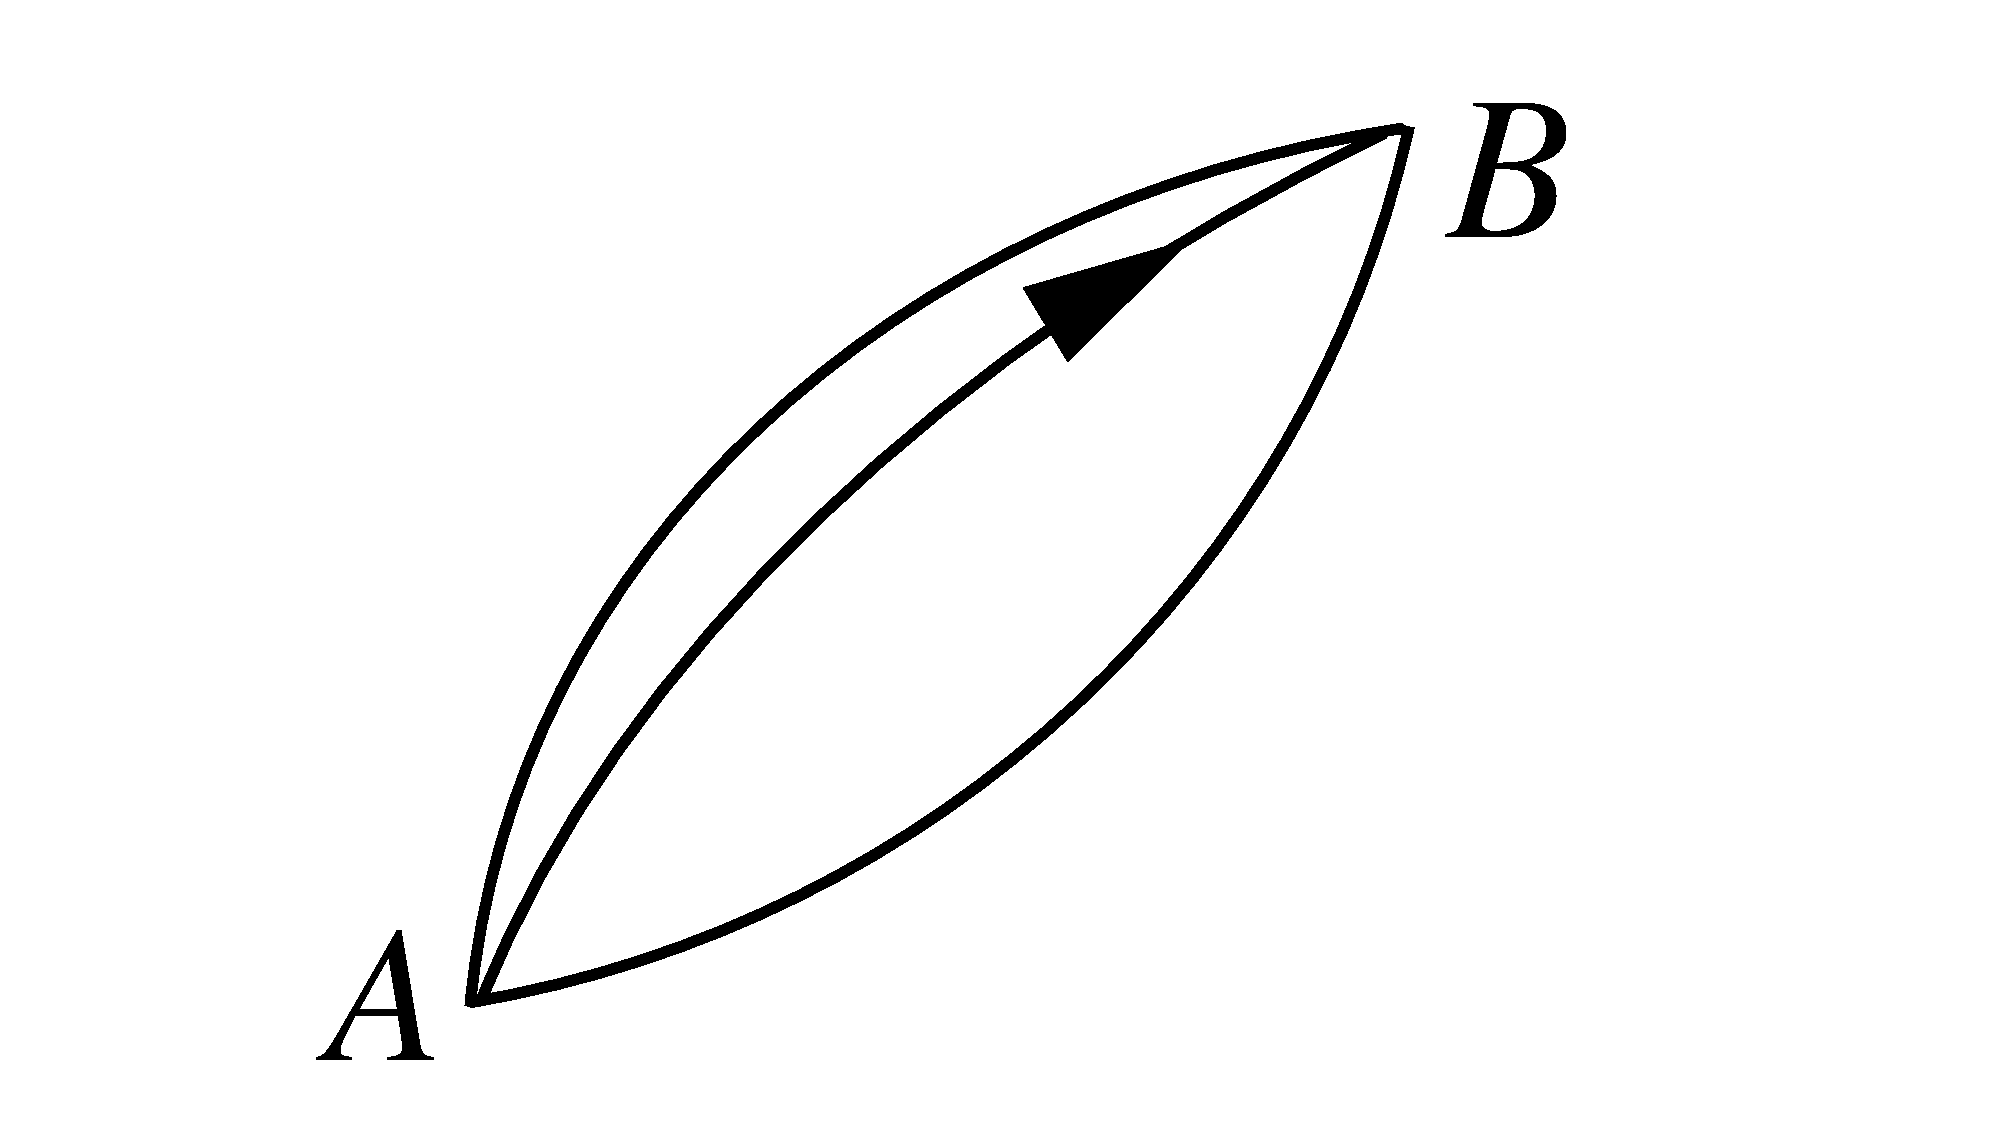
\includegraphics[width=2.5cm,clip]{QM file/figure/1-7}
	\caption{}
	\label{fig.1-7}
\end{wrapfigure}
其$m,p,E,V$表示质点的质量,动量,总能和势能,$\int pdl$称为作用量,质点由A至B的实际路径是作用量最小的路径.

德布罗意注意到光的本质包含者粒子和波动两个方面,光具有量子化的结构,每个光子具有一定的能量和动量:
\begin{equation}\label{eq15.3}
	E=\hbar\omega,\quad p=\frac{h}{\lambda},\quad \boldsymbol{p}=\hbar\boldsymbol{k}\quad
	(k=\frac{2\pi}{\lambda})
\end{equation}\eqnormal
在传播过程中,光表现出波动性,干涉、衍射等现象就是波动性的典型特征.但在宏观尺度上光的传播可以用光线概念来表述,波动光学表现为几何光学,波动规律以类似于力学规律的形式表现出来.德布罗意认为,电子以及其他物质粒子也都应该具有波动$\sim$粒子二重性.电子在结构上的量子性已为汤姆孙荷质比实验(测量$\frac{e}{m_{e}}$)所证实,电子在宏观尺度的运动遵守牛顿质点力学的规律,这早已被实验肯定.德布罗意认为,电子运动规律本质上应该是波动规律,这种波动性只有在微观尺度(量级和波长接近的尺度)才能表现出来,而在宏观尺度则表现为牛顿力学规律.德布罗意认为爱因斯坦公式\eqref{eq15.3}也适用于一切物质粒子,它们的力学性质$(E,p)$和波动性质$(\omega,\lambda)$通过普朗克常数$\hbar$互相联系.
\begin{wrapfigure}[8]{r}{8em}
	\centering
	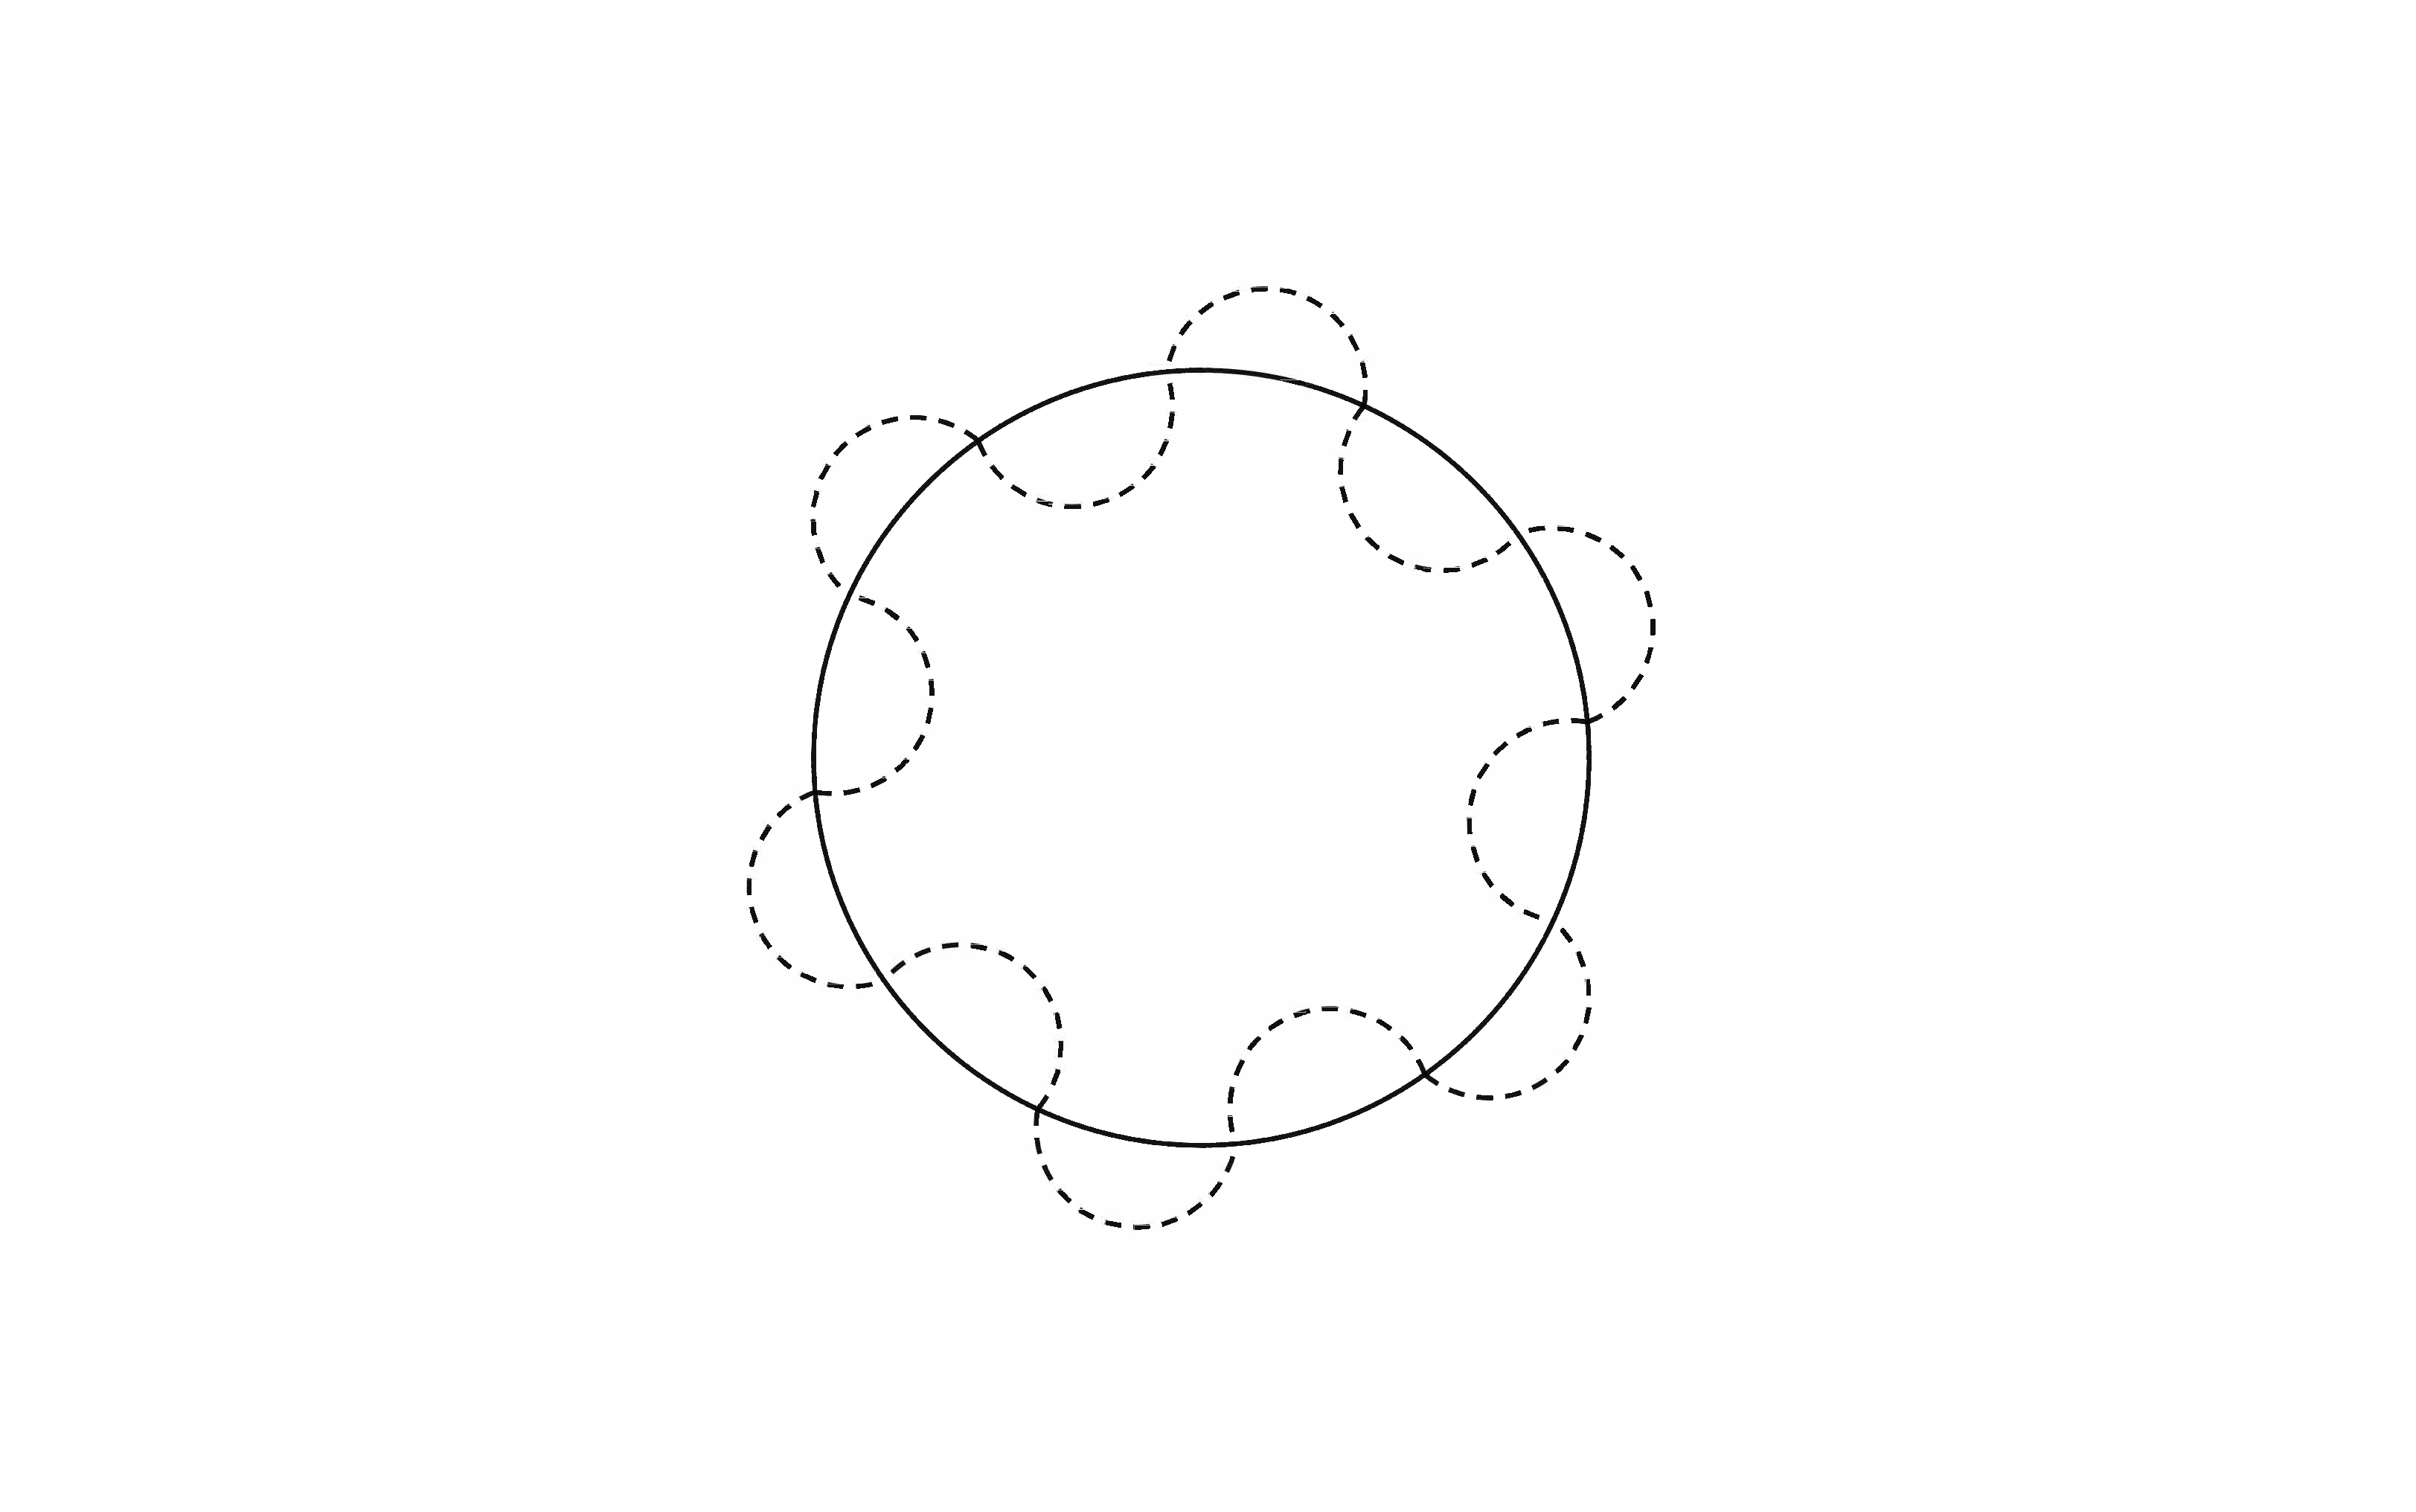
\includegraphics[width=2.5cm,clip]{QM file/figure/1-8}
	\caption{}
	\label{fig.1-8}
\end{wrapfigure}

德布罗意提出上述“物质波”设想时,并无直接的实验根据,而是一种科学假设.他希望这种未经证实的电子的波动性能够解释玻尔量子论所无法解释的那些困难问题.他指出,玻尔量子论中的量子化条件(这是玻尔理论中最难理解的一条)的实质很容易用波动的观点给以解释,如下.电子沿轨道运动,相当于物质波沿轨道传播,如果轨道周长不等于波长的整数倍,物质波将自行干涉而消失,亦即这种轨道是不允许的;如果轨道周长等于波长的整数倍,则物质波就能形成谐波而稳定存在,相应的轨道为稳定轨道形成谐波的条件为
\begin{equation}\label{eq15.4}
	\oint\frac{dq}{\lambda}=n,\quad n=1,2,3,\cdots	
\end{equation}
以$\lambda=\frac{h}{p}$代入上式,即得
\begin{equation}\label{eq15.5}
	\oint pdq=nh,\quad n=1,2,3,\cdots
\end{equation}
这正是量子化条件.

德布罗意的物质波思想直接导致了量子力学的诞生.相隔不到2年,薛定谔(E.Schr\"{o}dinger)就以“波动力学”的形式建立了量子力学(1926).稍早几个月,海森伯(W.Heisenberg)以“矩阵力学”的形式建立了量子力学(1925).

1927 年正式做了电子衍射实验,证实了电子确实具有波动性.接着又做了中子衍射实验,各种原子束和分子束的衍射实验,20世纪90年代还做了$C_{60}$分子(由60个碳原子形成的足球状大分子)束衍射实验,这些实验无一例外地都证实了公式$p=\frac{h}{\lambda}$的正确性,证实了实物粒子确实具有波动性.

当实物粒子在某种尺度的空间范围内运动时,如相应的物质波波长远小于空间尺度,一般可以不考虑粒子的波动性,而用经典力学处理粒子的运动.如波长接近或大于空间尺度,则波动性表现为粒子运动规律的主要方面,这时必须用量子力学来处理粒子的运动.下面举几个典型例子.

(1)气体分子的热运动.温度T下气体分子的热运动(平移)动能为$\frac{3kT}{2}$,$T=300 \si{K}$(室温)时,分子动能约为\num{0.039}\si{eV},相应的物质波波长为
\begin{equation*}
	\lambda=\frac{h}{p}=\frac{hc}{\sqrt{2m_{\text{分子}}\times\num{0.039}\si{eV}}}
\end{equation*}\eqshort
对于氧分子($O_{2}$),$m_{O_{2}}\approx32m_{p}\approx32\times938\times10^{6}\si{eV/c^{2}}$,波长$\lambda\approx0.026\si{nm}$,远小于分子的平均自由程,所以分子的热运动可作经典力学处理.

(2)原子中的电子运动电子动能的量级约10\si{eV},容易求得波长的量级为
\begin{equation*}
	\lambda\sim\frac{hc}{\sqrt{2m_{e}c^{2}E}}\sim 0.39\si{nm}
\end{equation*}\eqnormal
$\frac{\lambda}{2\pi}$和原子半径量级(0.1\si{nm})相同,所以要用量子力学来处理.

氢原子的基态,电子动能和动量为
\begin{equation*}
	\frac{p^{2}}{2m_{e}}=\frac{\e^{2}}{2a_{0}},\quad \boldsymbol{p}=\sqrt{\frac{m_{e}\e^{2}}{a_{0}}}=\frac{m_{e}\e^{2}}{\hbar}=\frac{\hbar}{a_{0}}
\end{equation*}\eqshort
波长为
\begin{equation*}
	\lambda=\frac{h}{p}=2\pi a_{0}
\end{equation*}\eqnormal
$a_{0}$为玻尔半径.

(3)原子核中核子的运动.核子(质子和中子)的动能约为$E\sim20 \si{MeV}$,相应的波长约为

\begin{equation}
	\begin{aligned}
		\lambda &\sim \frac{hc}{\sqrt{2m_{p}c^{2}E}}	\notag \\
				&\sim \frac{1.24\times10^{3} \si{MeV\cdot fm}}{\sqrt{2\times938\times20(\si{MeV})^{2}}}
				\approx 6.4 \si{fm}. \notag
	\end{aligned}
\end{equation}
核子的物质波波长$\lambda$和原子核半径同数量级,所以核子的运动也要用量子力学来处理.

% 习题
\begin{exercises}

\exercise 远离恒星的宇宙空间充满了温度$T=2.8\si{K}$的热辐射(称为宇宙背景辐射),这是宇宙发展早期“大爆炸"的遗迹. 试估算这种“背景辐射”的光子数密度.

\exercise 在宇宙发展的早期,温度极高,热辐射光子互相碰撞,可以转变成一对正负电子.试估算当时温度的量级.

\exercise 对于光子被自由电子散射(康普锁散射)问题,设光子能量远小于$m_{e}c^{2}$,则散射过程中电子的能量、动量变化可以用牛顿力学处理.试作出相应的计算,求光的波长变化与散射角的关系.

\begin{wrapfigure}[6]{r}{10em}
	\centering
	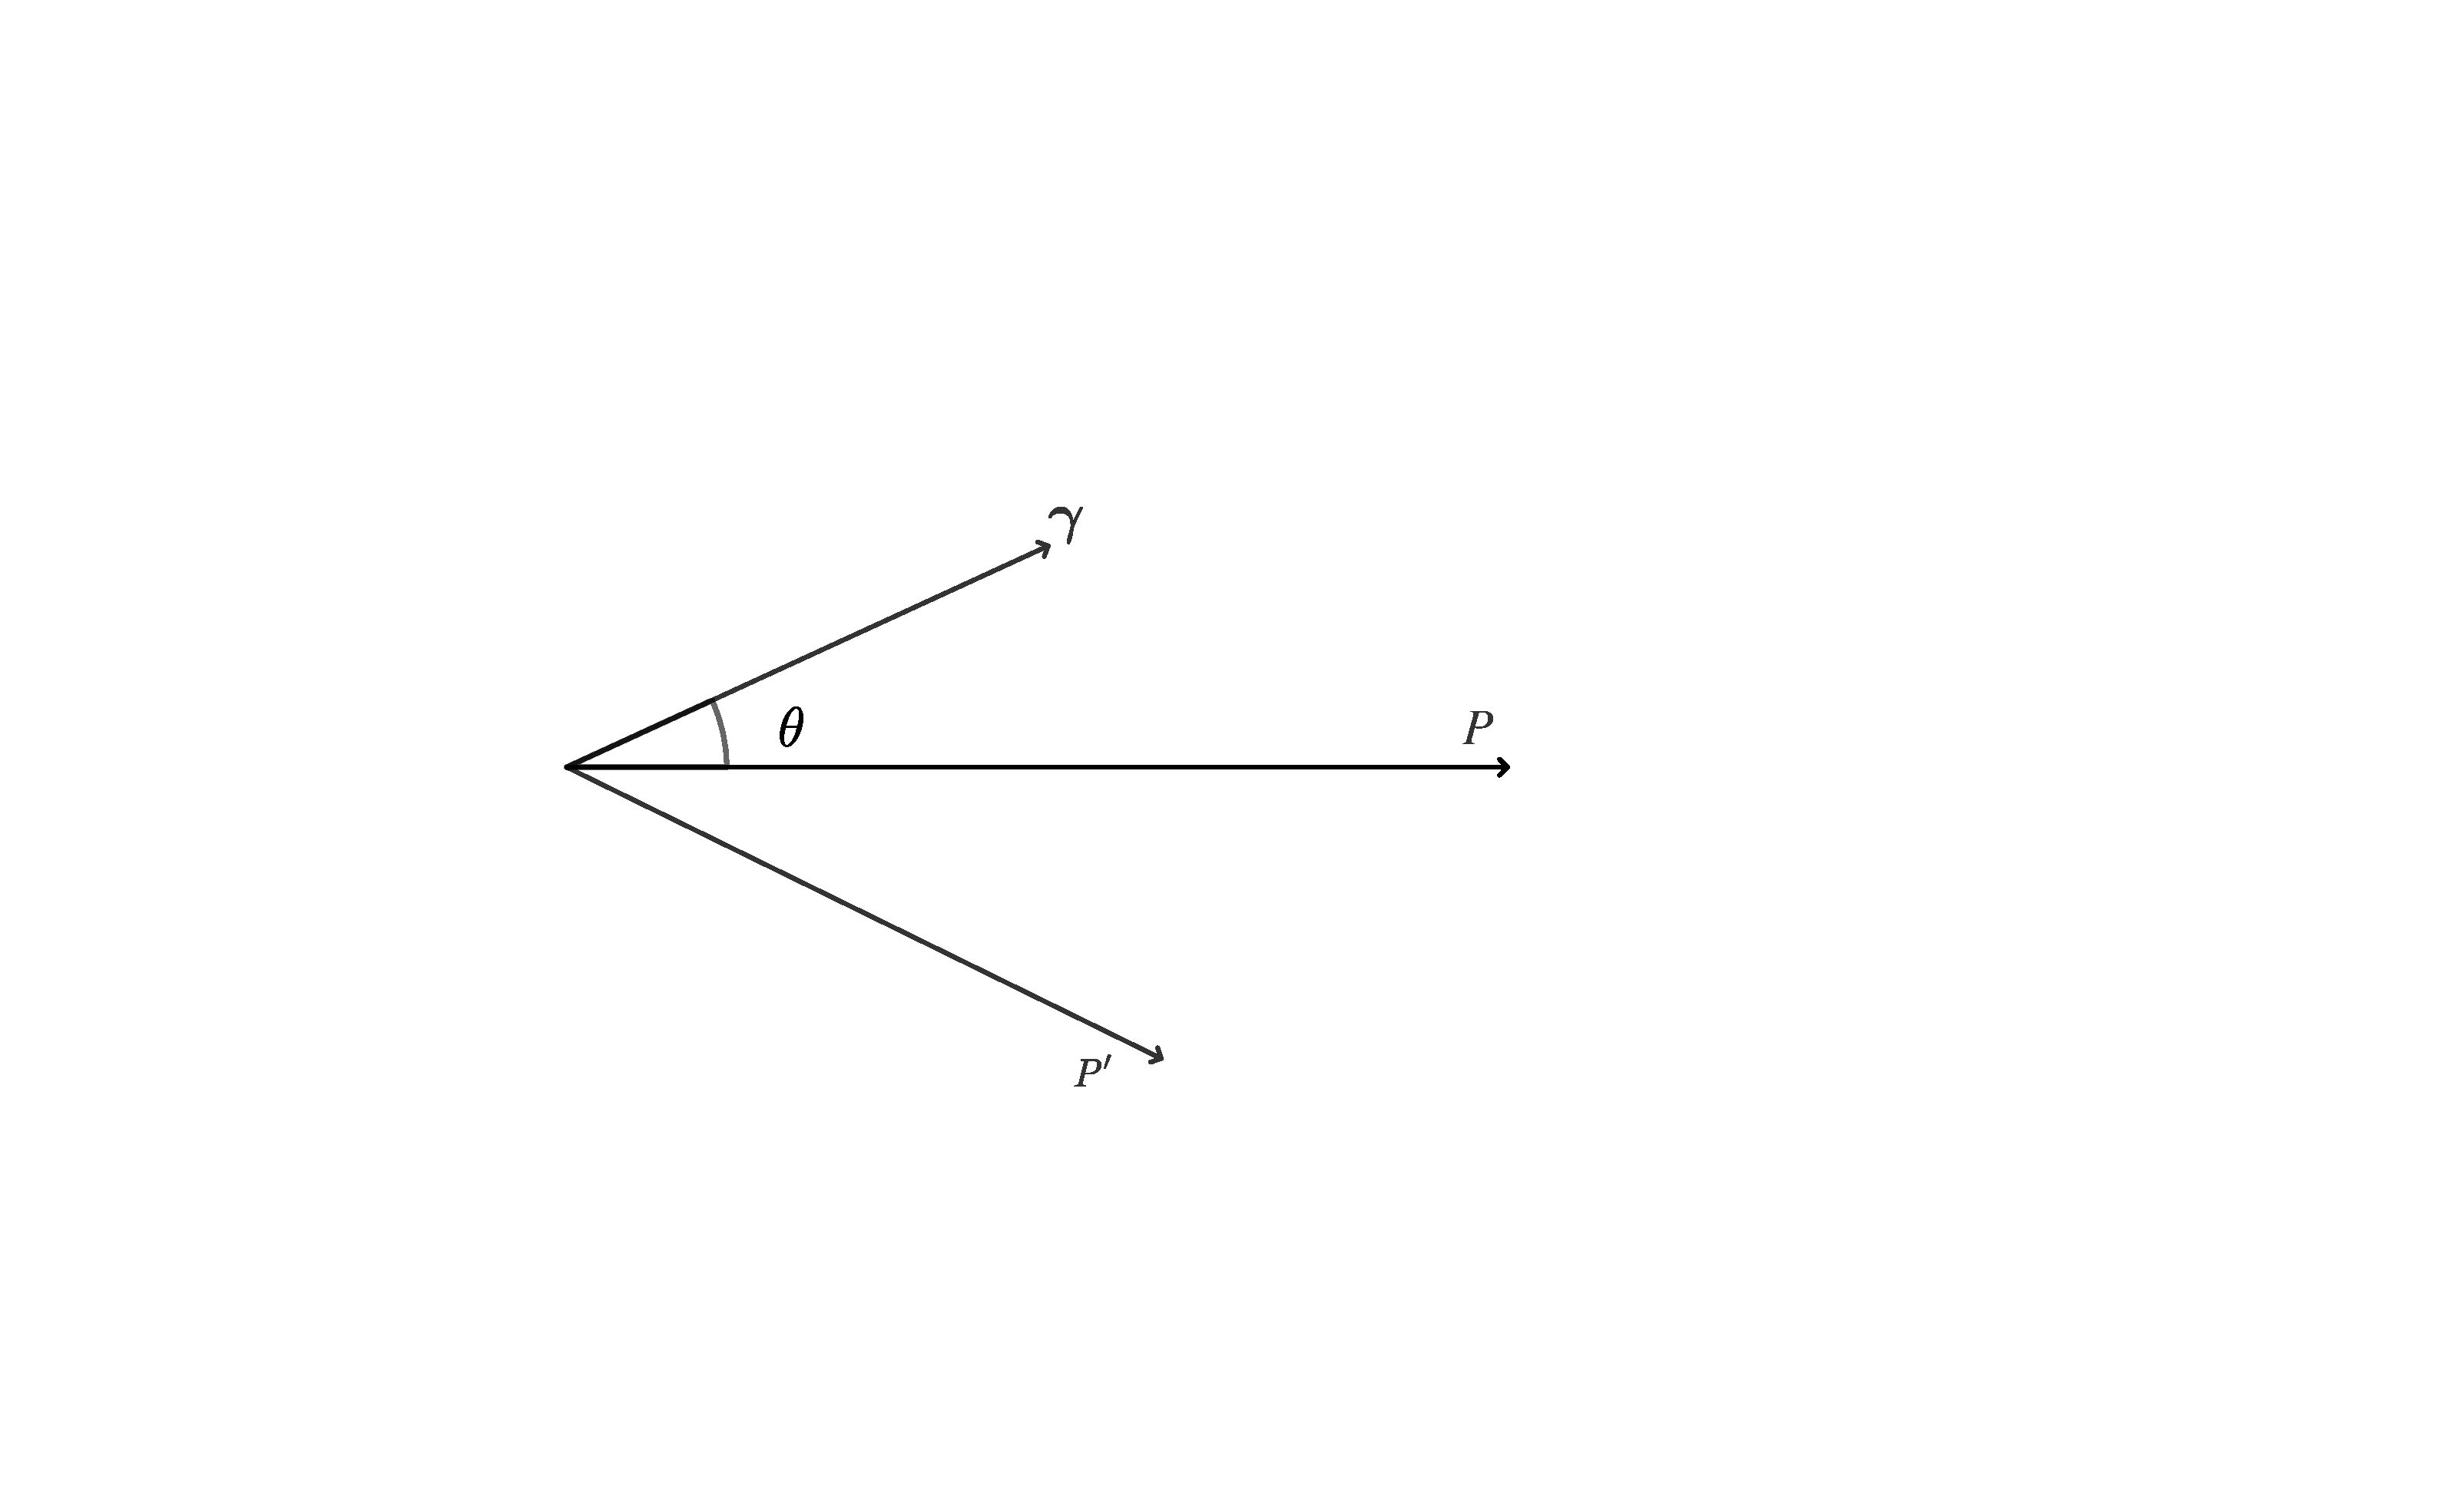
\includegraphics[width=3.5cm,clip]{QM file/figure/1-9}
	\caption{1-4题图}
	\label{fig.1-9}
\end{wrapfigure}
\exercise 高能带电粒子在介质中运动,如其速度$v$超过电磁波在介质中的传播速度,就产生切仑科夫辐射.设介质的折射率为$n$,辐射光与粒子运动方向的夹角为$\theta$.试利用光子的能量,动量公式($E_{\gamma}=\hbar\omega,p_{\gamma}=\hbar k$)以及能量守恒及动量守恒定律,求$\theta$与$n,v$的关系

$\big[\text{提示:光在介质中传播时,}\omega=\dfrac{ck}{n}. \big]$

\exercise 从质量为$m$,半径为$R$的星球表面辐射出频率为$\nu_{0}$的光,当这种光在远离星球处被观测到时,测得的频率$\nu<\nu_{0}$,这种现象称为恒星光谱的“引力红移”.设光子可以当作“质点”,引力质量$m_{\text{光}}=\dfrac{h\nu}{c^{2}}$下,光子离开星球时,必须克服星球对它的万有引力.试根据这种通俗模型导出$\dfrac{\nu}{\nu_{0}}$的公式.

\exercise 来自其他恒星的光掠过太阳(质量$M$,半径$R$)表面时,光线方向发生微小的偏转($\theta$).这个现象曾是广义相对论的实验支柱之一.试利用$1\sim 5$题中光子的“质点”模型对偏转角$\theta$作出量级估算.
\begin{figure}[!h]
	\centering
	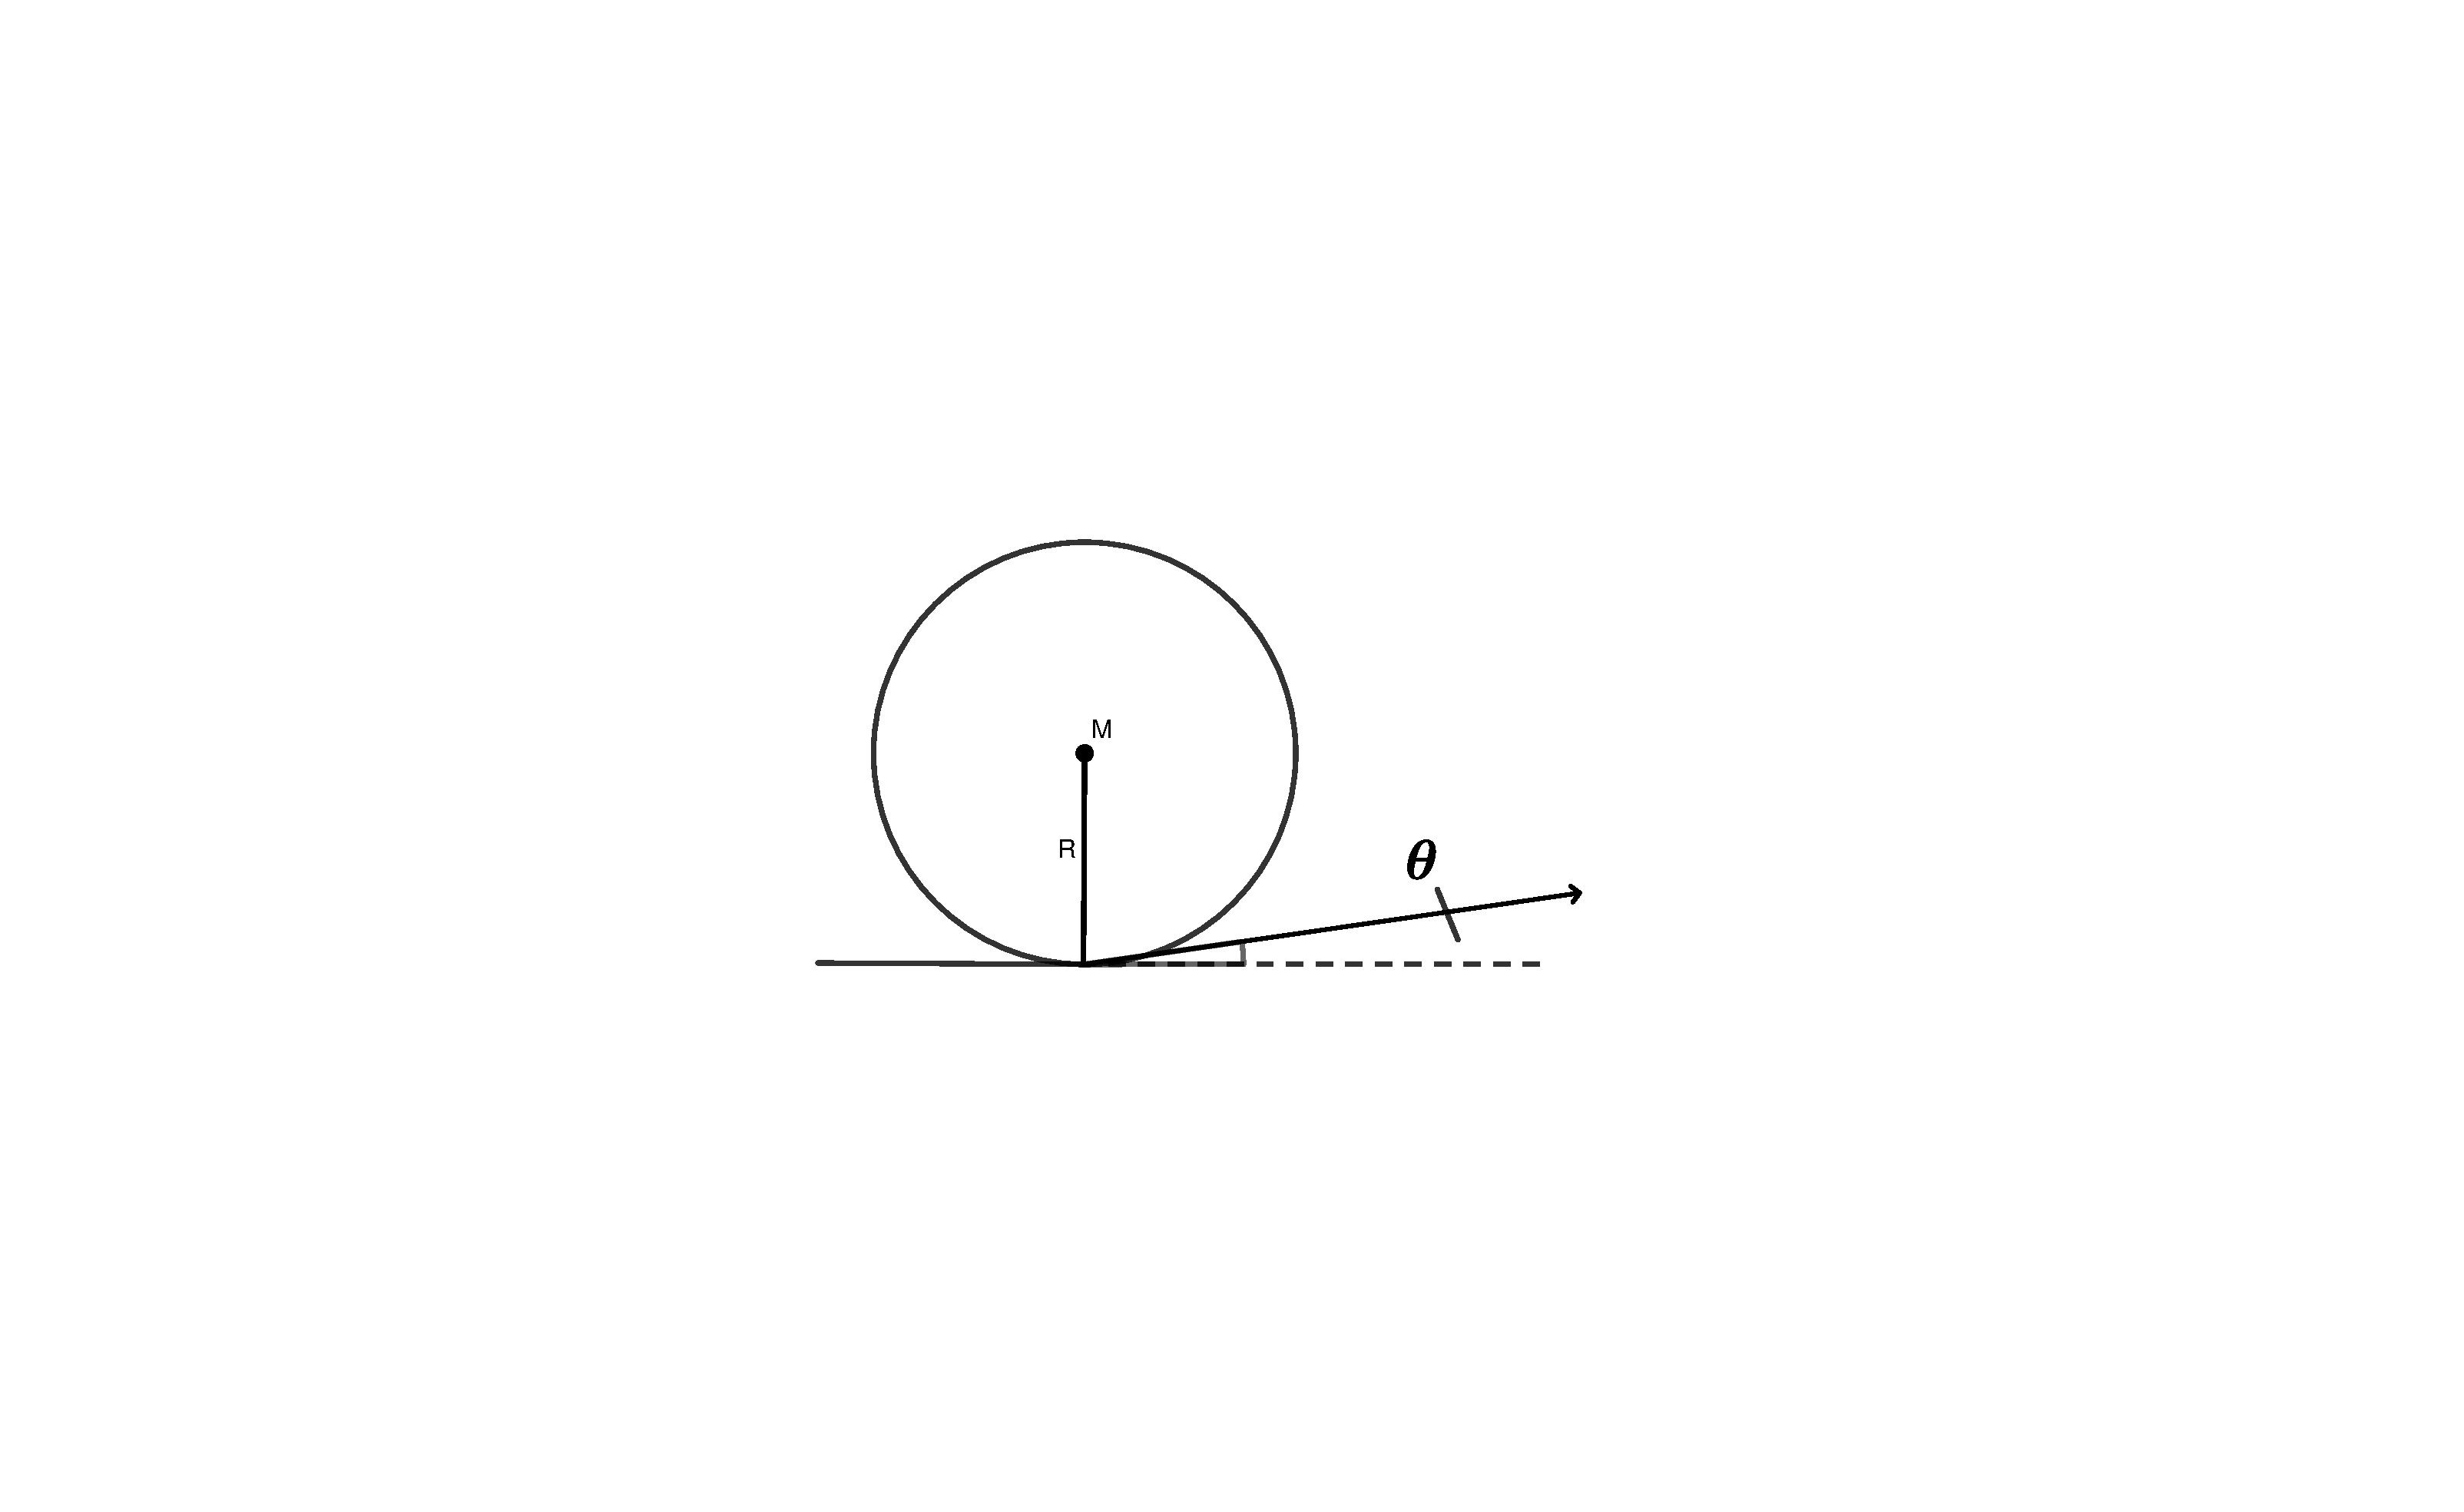
\includegraphics[width=3.5cm,clip]{QM file/figure/1-10}
	\caption{1-6题图}	\label{fig.1-10}
\end{figure}
\exercise 氢原子中电子-质子间库仑吸引力远大于万有引力.求这两种力的比率.理论上,电子与中子间的万有引力也可以使它们形成类似于氢原子的构造,试求这种“引力原子” 的基态半径公式及数值.

\exercise (a) $\mu^{-1}$子电荷为$-e$,质量$m_{\mu}=207m_{e}$,$\mu^{-1}$子与原子核(电荷$Ze$)由于库仑吸引力的作用而形成类似氢原子的构造.称为$\mu$原子.视原子核为点电荷,求$\mu$原子半径公式.
	
\quad (b) 原子核可视为电荷均匀分布的球体, 核半径的经验公式为
\begin{equation*}
	R=r_{0p}Z^{1/3},\quad r_{0p}=1.635\si{fm}
\end{equation*}
对于较大的原子序数$Z$,核半径$R$有可能大于$\mu$原子半径.求出现这种情况的$Z$的临界值$Z_{0}$. 

\exercise 计算原子核(电荷$Ze$,半径$R$)中各质子间库仑排斥能的总和及(按质子)平均值.原子核半径公式见1-8题.当$Z$取多大数值时,每个质子的平均库仑能达到核力结合能(每个核子约8\si{MeV})的量级?

\exercise 电子自旋磁矩等于$\mu_{B}$=$\dfrac{\e\hbar}{2m_{\e}c}$(玻尔磁子).在磁场$(B)$中电子获得的磁作用能大致为$B\mu_{B}$量级.如$B\mu_{B}\sim10^{-3}\si{eV}$,求磁场$B$的量级.

\exercise 估算氢分子转动能级的“解冻温度”.氢分子键长$R=0.74\times10^{-8}\si{cm}$.

\exercise 由于电磁场的真空量子效应,两块相隔距离$d$的不带电大导体平板间产生微弱吸引力设单位面积受力F,试用量纲分析法确定$F$与各基本普适常数及距离$d$的关系.

\exercise { (a) 求室温(T=300 \si{K})下中子的德布罗意波长.
	
	\quad (b) 如上述中子在地面附近垂直下落1\si{m},求波长变化的比率.
}

\exercise 如普朗克常数的值变成现有值的2倍,而其他基本常数之值不变,下列各项数值变为现有值的多少倍?

(a)原子半径 \quad (b)晶体密度 \quad (c)蓄电池的电压

\exercise 质量为$m$的粒子受弹性力$F=-kx(k>0)$作用而作一维简谐振动,按照经典力学可以求出其运动规律为
\begin{equation*}
	x(t)=A\sin(\omega t+\alpha),\quad \omega=\sqrt{\frac{k}{m}}
\end{equation*}
A为振幅谐振子的能量为$E=\dfrac{1}{2}kA^{2}$.以上请读者自行验证.试再利用玻尔-索末菲量子化条件或对应原理证明能量及振幅的量子化结果:
\begin{equation*}
	E_{n}=n\hbar\omega,\quad A_{n}=\sqrt{\frac{2n\hbar}{m\omega}},\quad n=0,1,2,\cdots
\end{equation*}
$\big[$提示:宏观的谐振动电荷,辐射的电磁波频率与振动频率相同.据此,再利用对应原理,很容易得出结论.$\big]$

\exercise 质量为$m$的粒子在大小一定的向心力$\boldsymbol{F}=-\dfrac{k\boldsymbol{r}}{r}$作用下作圆周运动.先用经典力学证明轨道半径$r$,角速度$\omega$,总能量$E$有如下关系:
\begin{equation*}
	r\omega^{2}=\frac{k}{m},\quad \boldsymbol{E}=\frac{3}{2}k\boldsymbol{r}=\frac{3}{2}\frac{k^{2}}{m\omega^{2}}
\end{equation*}
再利用量子化条件或对应原理证明能级的量子化公式:
\begin{equation*}
	E_{n}=\frac{3}{2}\bigg(\frac{\hbar^{2}k^{2}n^{2}}{m} \bigg)^{\frac{1}{3}},\quad n=1,2,3,\cdots
\end{equation*}
 
\end{exercises}

